\section{概览}
\label{sec:appendix_overview}
本补充材料提供更多结果以补充主文。
首先，我们在~\cref{sec:details} 中给出包括网络架构在内的全部实现细节。
随后，我们在~\cref{sec:training_details} 中详细说明 FoV 采样和数据集等训练细节。
接着，我们在~\cref{sec:class_agnostic} 中描述如何执行类别无关实例分割。
最后，我们在~\cref{sec:more_qualitative} 中提供视频对象跟踪和类别无关实例分割的更多定性比较。
除本文档外，我们还提供额外视频结果，用于与最先进方法进行比较。


\section{实现细节} \label{sec:details}
由于计算资源限制，所有实验均使用 SAM~2.1-Large 作为基线。Hiera~\cite{ryali2023hiera} 图像编码器产生多尺度特征，其中 stride-16 和 stride-32 输出（Stages 3/4）通过带卷积的 FPN~\cite{lin2017featureFPN} 融合以获得帧嵌入；而来自 Stages 1/2 的浅层特征（stride 4/8）仅注入掩码解码器，用于恢复精细边界。记忆注意力使用正弦绝对位置嵌入与 2D RoPE；对象指针 token 不使用 RoPE，并且我们采用 $L=4$ 层。提示编码器遵循 SAM，掩码解码器将 mask token 作为存储在记忆库中的对象指针。额外 token 通过 MLP 头预测对象可见性，遮挡帧则在记忆中接收一个学习到的遮挡嵌入。与 SAM~2 类似，当存在歧义时，解码器输出多个候选掩码并选择预测 IoU 最高者。记忆编码器复用 Hiera 特征，无需单独骨干网络；记忆特征被投影到 64 维，256 维指针被拆分为四个 64 维 token 用于交叉注意力。对于多对象视频，图像编码器共享，而每个对象维护独立的记忆库和解码器。
 
\subsection{Feature Merger}


如 \cref{fig:feature_merging} 所示，我们的方法使用来自 MUSt3R 解码器的多层特征。
我们保持 MUSt3R 的记忆机制不变，即不修改其基于视角覆盖的记忆选择。
我们根据经验选择层索引 $[\text{encoder}, 4, 7, 11]$，以同时引入早期层的语义线索和后期层的几何感知信号，因为 MUSt3R 中更深的解码器层会逐渐捕获 3D 结构并直接解码点云。

选择 MUSt3R 特征后，我们使用一系列交叉注意力操作将其融合。
我们首先构造位置嵌入：PE3D 通过处理 MUSt3R 产生的点图和射线图得到，而 PE2D 取自 MUSt3R 的 2D 位置编码。
编码器特征通过 $1\!\times\!1$ 卷积从 1024 通道投影到 768 通道，与 PE3D 相加后，再经过带 PE2D 的自注意力层，形成初始粗特征 $F_{\text{coarse}}$。

对于每个选中的 MUSt3R 层 $F_i$（$i \in \{4,7,11\}$），我们使用如下方式更新 $F_{\text{coarse}}$：
\begin{equation} \small
\resizebox{\columnwidth}{!}{$
F_{\text{coarse}}
\leftarrow
\mathrm{FFN}\!\left(
\mathrm{CrossAttn}\!\big(
\mathrm{SelfAttn}(F_{\text{coarse}} + \mathrm{PE3D}),
\, F_i + \mathrm{PE3D}
\big)\right).
$}
\end{equation}
为清晰起见，我们省略归一化和跳跃连接。

注意力融合后，$F_{\text{coarse}}$ 经过上采样和 $3\!\times\!3$ 卷积细化，随后与 SAM~2 中 Hiera 图像编码器特征 $F_{2D}$ 拼接，并通过额外卷积块匹配特征维度。
得到的特征 $F_{\text{merged}}$ 用于记忆注意力和记忆编码。
我们保持 Stages~1 和~2 的浅层 Hiera 特征不变，使掩码解码器仍可依赖强低层视觉线索生成高分辨率分割输出。


\section{训练细节} \label{sec:training_details}
\subsection{Field-of-View Sampling}
我们不使用 100\% FOV 感知采样，因为观察到对每个 batch 都应用 FOV 过滤会削弱模型从 SAM2 继承的原始特征匹配能力。
当所有训练样本都来自差异剧烈的视角时，模型会被过度正则化到跨视角匹配，并失去视角内对应能力，从而产生某种形式的特征塌缩。  



% }
\subsection{设置}

\paragraph{损失}
我们不加修改地遵循 SAM2 的损失设计。
具体而言，掩码预测使用 focal loss（20）和 dice loss（1）的加权组合进行监督；
IoU 头使用 $\ell_{1}$ 损失（1）训练；
遮挡预测头使用交叉熵损失（1）。

\paragraph{提示}
由于退化的 2D 掩码以及训练采样策略引入的大幅视角变化，对于 ScanNet++ 和 ASE，我们将输入模态限制为仅使用掩码。对于 MOSE，我们启用所有提示类型，包括点、框和掩码输入。

\subsection{数据集}
\paragraph{Aria Synthetic Environments (ASE)~\cite{avetisyan2024scenescript}}
ASE 是一个大规模合成数据集，包含 100,000 个由程序生成并使用模拟 Aria 眼镜传感器渲染的室内场景。每个场景包含真实感 3D 对象布局、模拟轨迹以及对齐的 2D/3D 标注。
ASE 支持 3D 场景理解、对象检测和跟踪的大规模训练，尤其适用于真实标注数据稀缺而数据需求较高的设置。
我们总共采样 2{,}612 个视角数量处于实用范围内的场景：
视角过少的场景无法为训练提供足够视角变化，
而视角过多的场景在运行 MUSt3R 时会导致内存溢出。

\paragraph{MOSE~\cite{MOSE}}
MOSE 数据集（Complex Video Object Segmentation）面向杂乱且存在遮挡的真实场景中的视频对象分割。它包含 2,149 个视频片段、来自 36 个类别的 5,200 个对象，以及 431,725 个高质量掩码。
不同于以往包含大型、显著、孤立目标的 VOS 基准，MOSE 包含严重遮挡、对象消失与重现，以及小型/不显眼对象。
MOSE 主要用于保持模型的核心 VOS 能力。
虽然我们的几何整合鼓励强跨视角一致性，但我们不希望模型过度依赖几何，并在缺乏足够视觉证据时“幻觉”出对象轨迹；MOSE 有助于将模型锚定在外观驱动线索上。  

尽管 MUSt3R 支持动态场景，我们发现，在 SA-V Train 等高度动态且多样的数据集上训练在实践中会导致不稳定。MOSE 提供了更可控的运动和场景变化程度，使我们能够在利用动态对象监督的同时保持稳定学习。


\paragraph{ScanNet++~\cite{yeshwanth2023scannet++}}
ScanNet++ 是一个高质量室内 RGB--D 重建数据集，提供精确相机位姿、稠密轨迹和详细几何标注。
公开版本包含超过 1{,}000 个重建场景，是初始较小版本的扩展\cite{yeshwanth2023scannet++}。
可靠几何与视角多样性的结合，使其非常适合研究大幅相机运动下的视角一致对象跟踪。
然而，ScanNet++ 中的 2D 掩码由 3D 点云实例标签投影到图像平面生成，不可避免地会因深度和位姿不准确引入重投影噪声。此外，ScanNet++ 的位姿标注常会缺失长段连续帧，因为 SfM 流程会丢弃不确定帧。在这种条件下，我们基于 FoV 的采样变得更加重要。
尽管如此，ScanNet++ 仍然很有价值，因为它提供具有丰富几何结构和大幅视角变化的真实室内场景。
结合另外两个提供干净、帧对齐 2D 掩码的数据集，它形成了一个互补训练组合，在真实几何和高质量外观监督之间取得平衡。



\section{类别无关实例分割} \label{sec:class_agnostic}

对于类别无关 3D 实例分割，我们按如下方式处理。
给定一组关键帧（按固定间隔采样，或使用视角覆盖准则选择），我们首先使用 SAM2 自动掩码生成器生成 2D 实例掩码。
对于每个关键帧 $i$，随后使用我们的模型将其实例掩码向前传播到所有后续帧；不执行反向跟踪。
传播后的掩码通过深度图和相机位姿对其像素反投影，被提升到 3D。
一个实际问题是对象边界附近存在重投影误差，这由深度噪声和视角相关错位导致。
为缓解该问题，我们 (1) 使用投影深度与真值深度之间的一致性计算重投影得分，(2) 在投影前轻微腐蚀 2D 掩码，从而减少集中在对象边缘附近的伪影。

获得逐帧 3D 片段后，我们将其合并为整合后的 3D 实例。
对于每个片段，我们计算两个得分：
(1) 点云域中的 3D 重叠得分；
(2) 基于视频中传播掩码的 2D 时间重叠得分。
由于我们的模型在视频中保持一致对象身份，先前可见的对象在重现时会被再次识别，从而为合并提供可靠时间证据。

最后，合并后通过超点级多数投票解决重复分配：每个超点被分配给其被观察次数最多的实例。





\begin{figure*}[t]
    \centering
    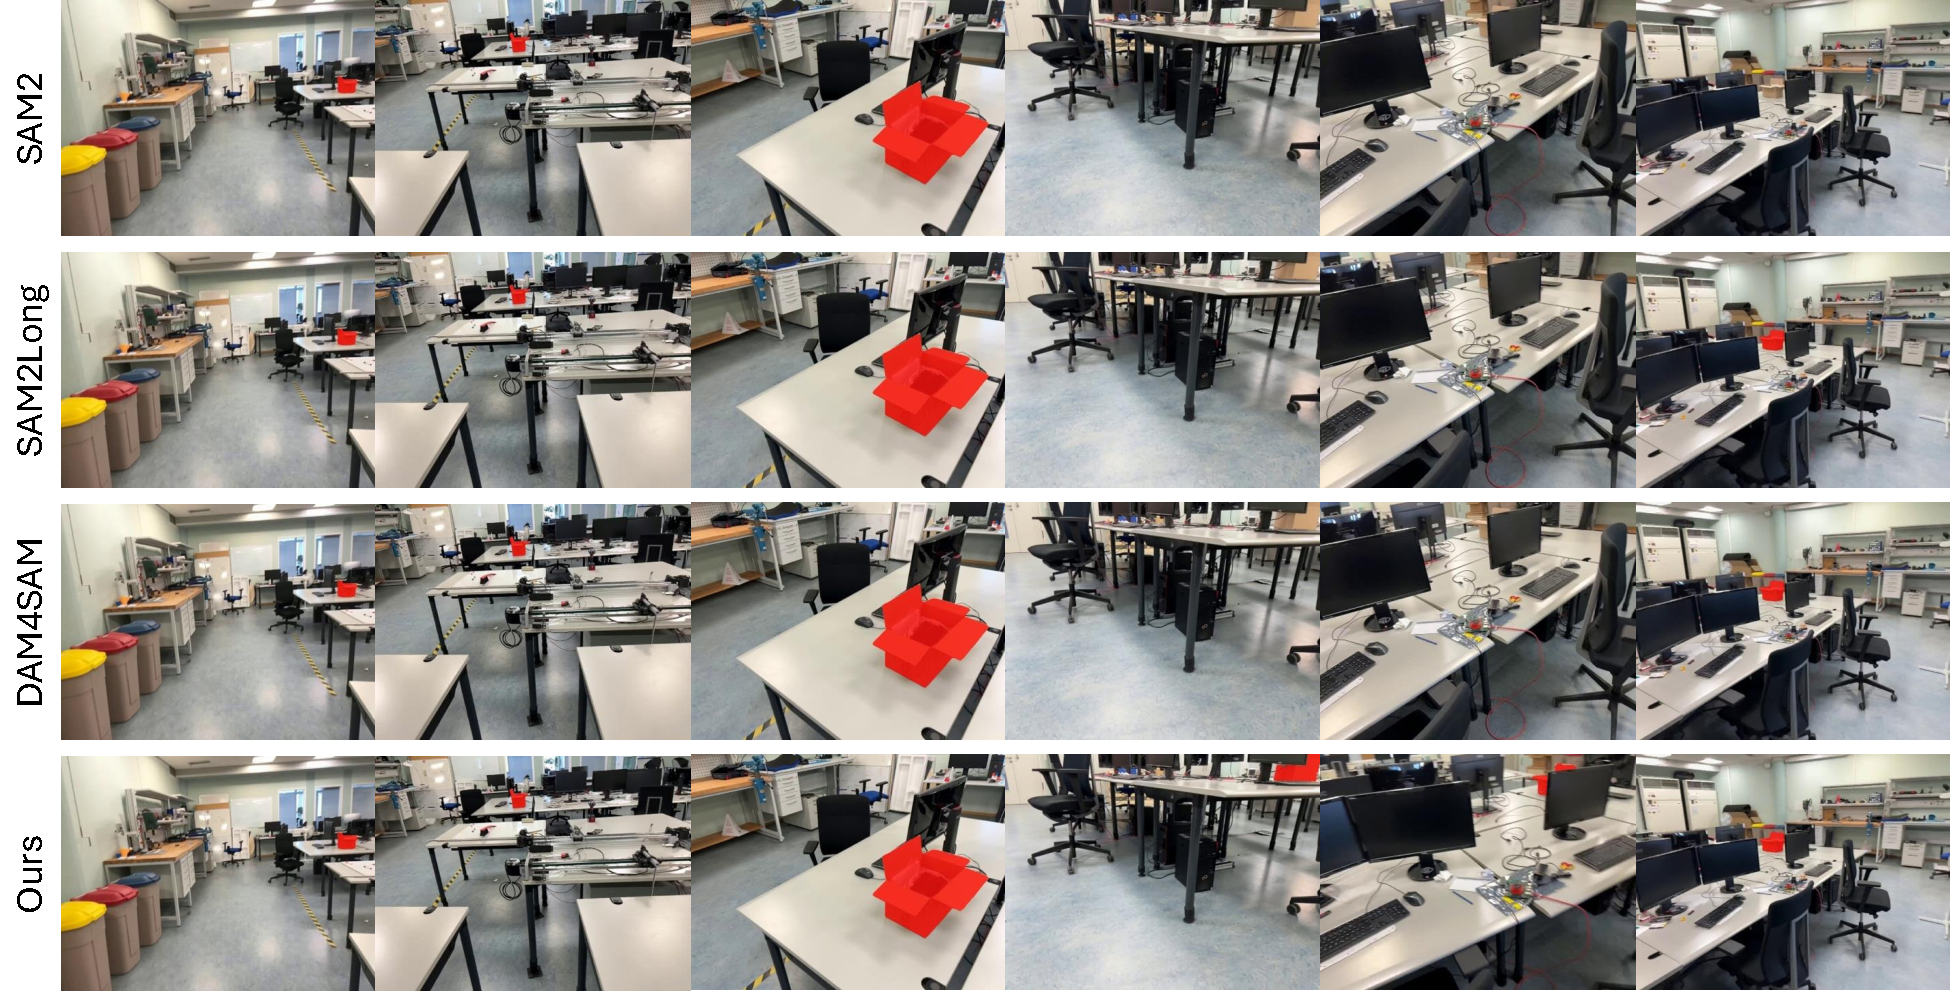
\includegraphics[width=1.0\textwidth]{figs/vis_comp.pdf}
    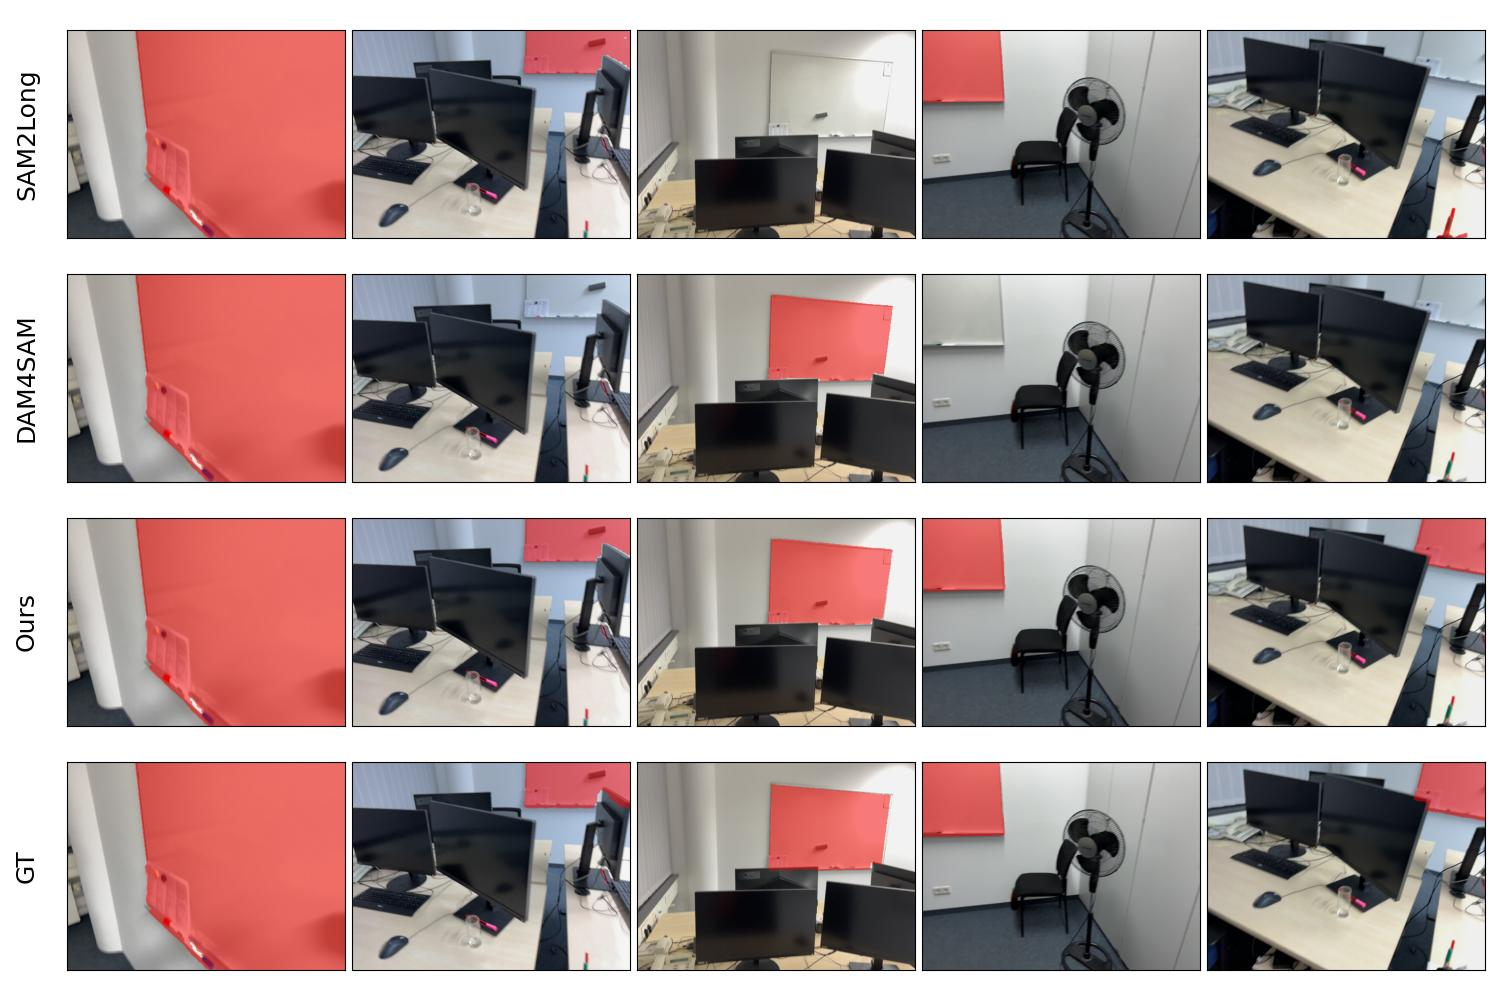
\includegraphics[width=1.0\textwidth]{figs/fig-vis/1ada7a0617/pred_masks_instance_512_7.jpg}
    \caption{
    \textbf{不同 VOS 方法的视觉比较}
    }
    \label{fig:vis_comp_app}
\end{figure*}

\begin{figure*}[t]
    \centering
    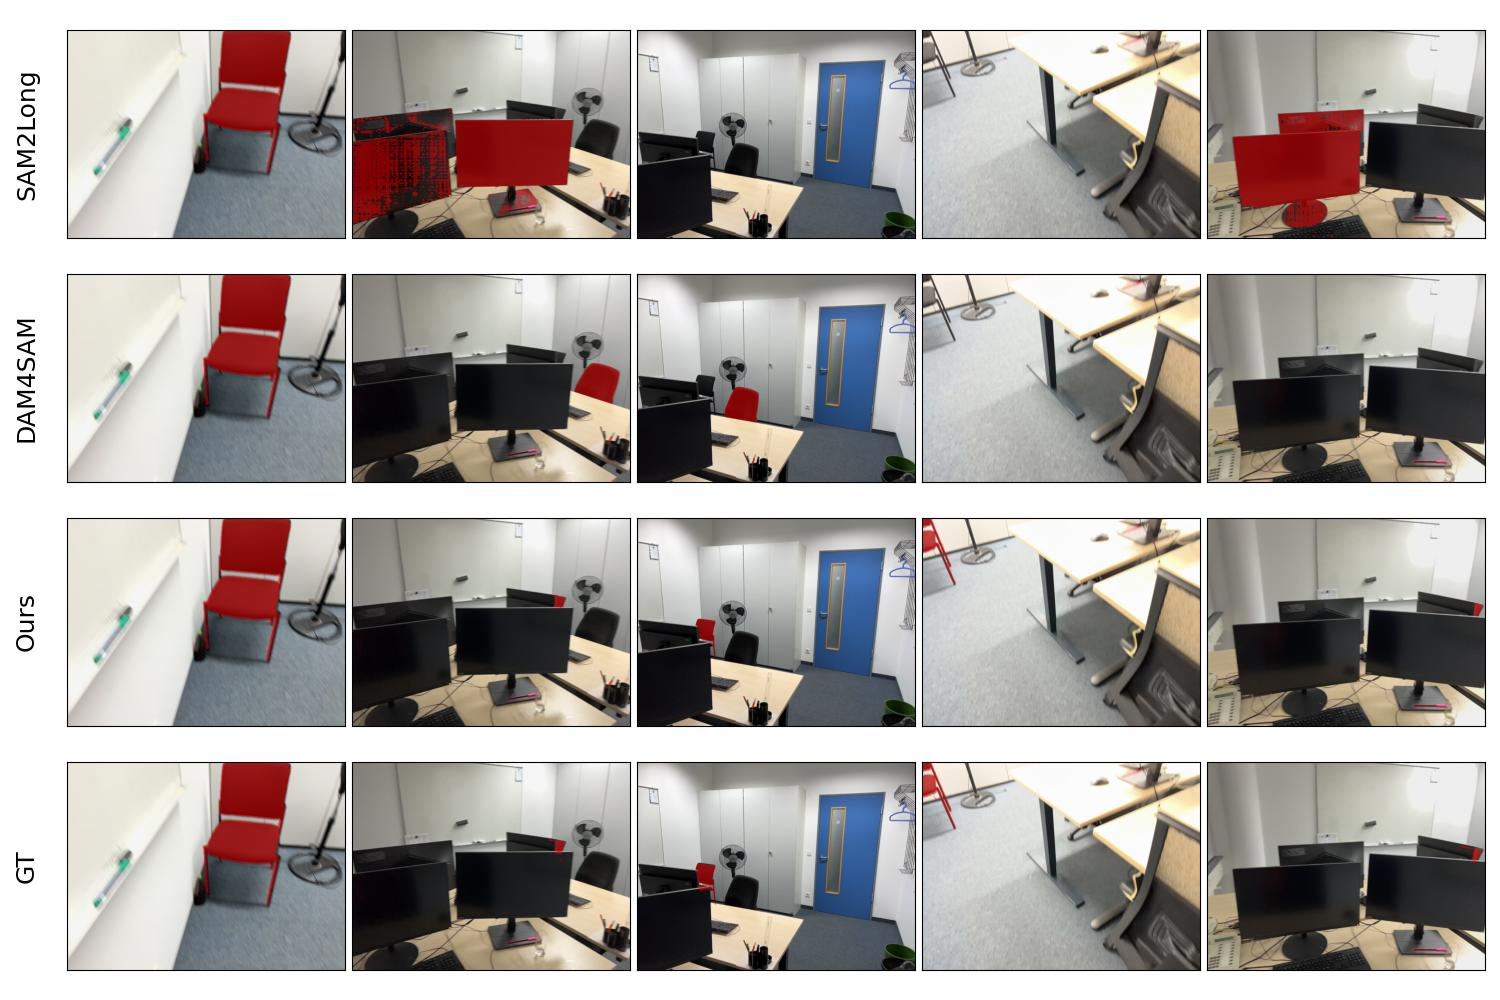
\includegraphics[width=1.0\textwidth]{figs/fig-vis/1ada7a0617/pred_masks_instance_512_11.jpg}
    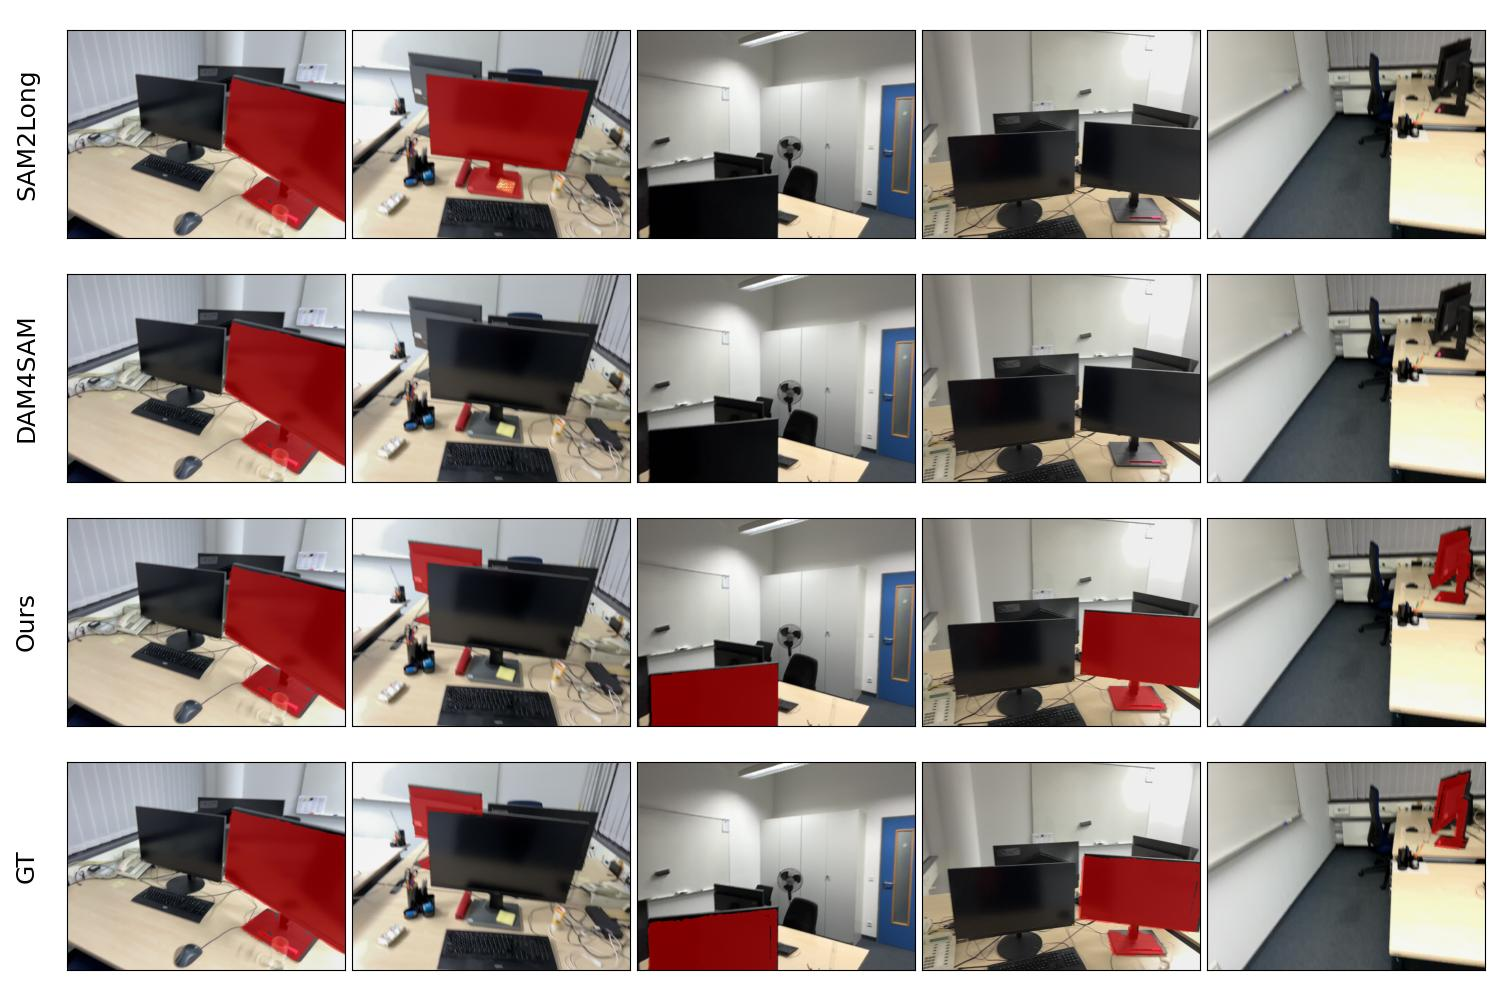
\includegraphics[width=1.0\textwidth]{figs/fig-vis/1ada7a0617/pred_masks_instance_512_36.jpg}
    \caption{
    \textbf{不同 VOS 方法的视觉比较}
    }
    \label{fig:vis_comp2}
\end{figure*}

\begin{figure*}[t]
    \centering
    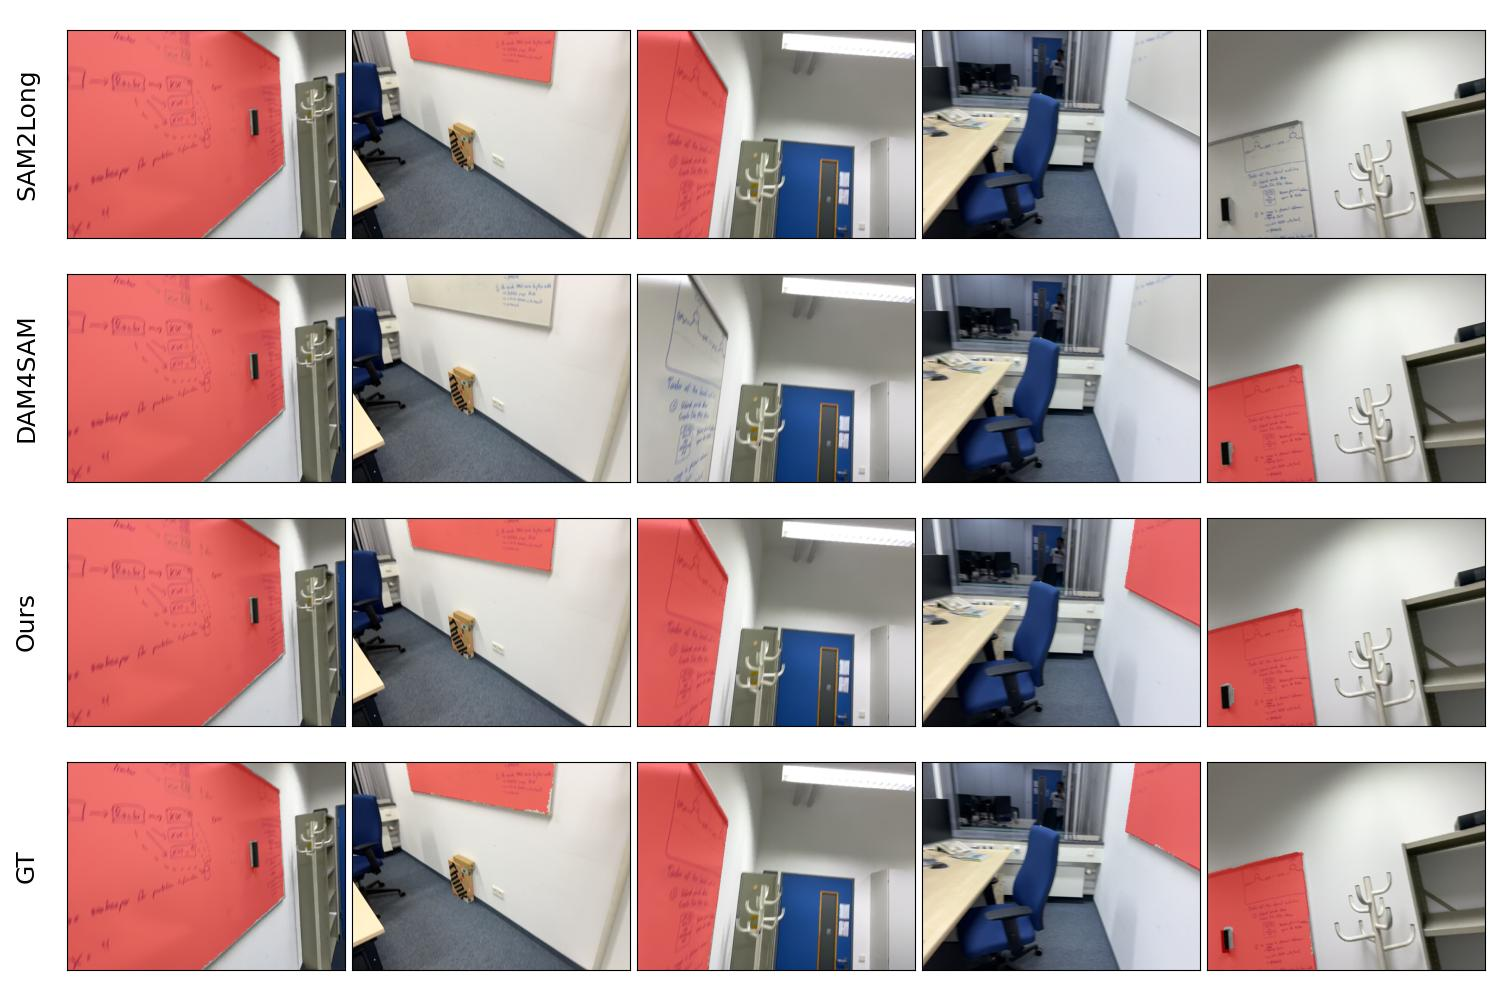
\includegraphics[width=1.0\textwidth]{figs/fig-vis/7b6477cb95/pred_masks_instance_512_10.jpg}
    
\includegraphics[width=1.0\textwidth]{figs/fig-vis/7b6477cb95/pred_masks_instance_512_11.jpg}
    \caption{
    \textbf{不同 VOS 方法的视觉比较}
    }
    \label{fig:vis_comp3}
\end{figure*}

\begin{figure*}[t]
    \centering
    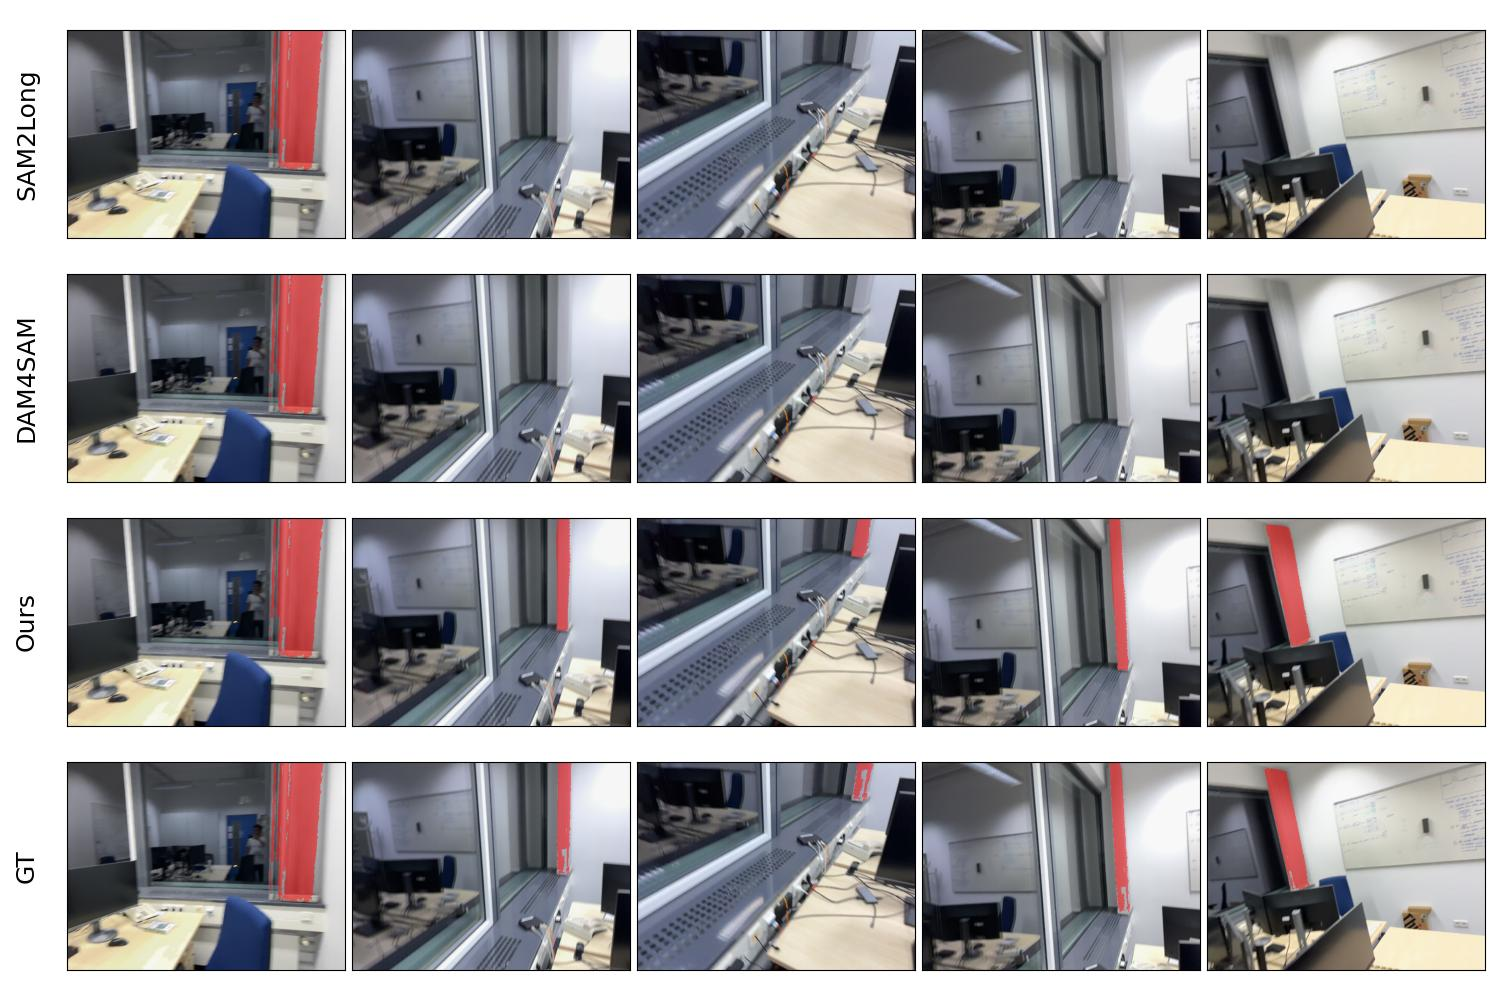
\includegraphics[width=1.0\textwidth]{figs/fig-vis/7b6477cb95/pred_masks_instance_512_45.jpg}
    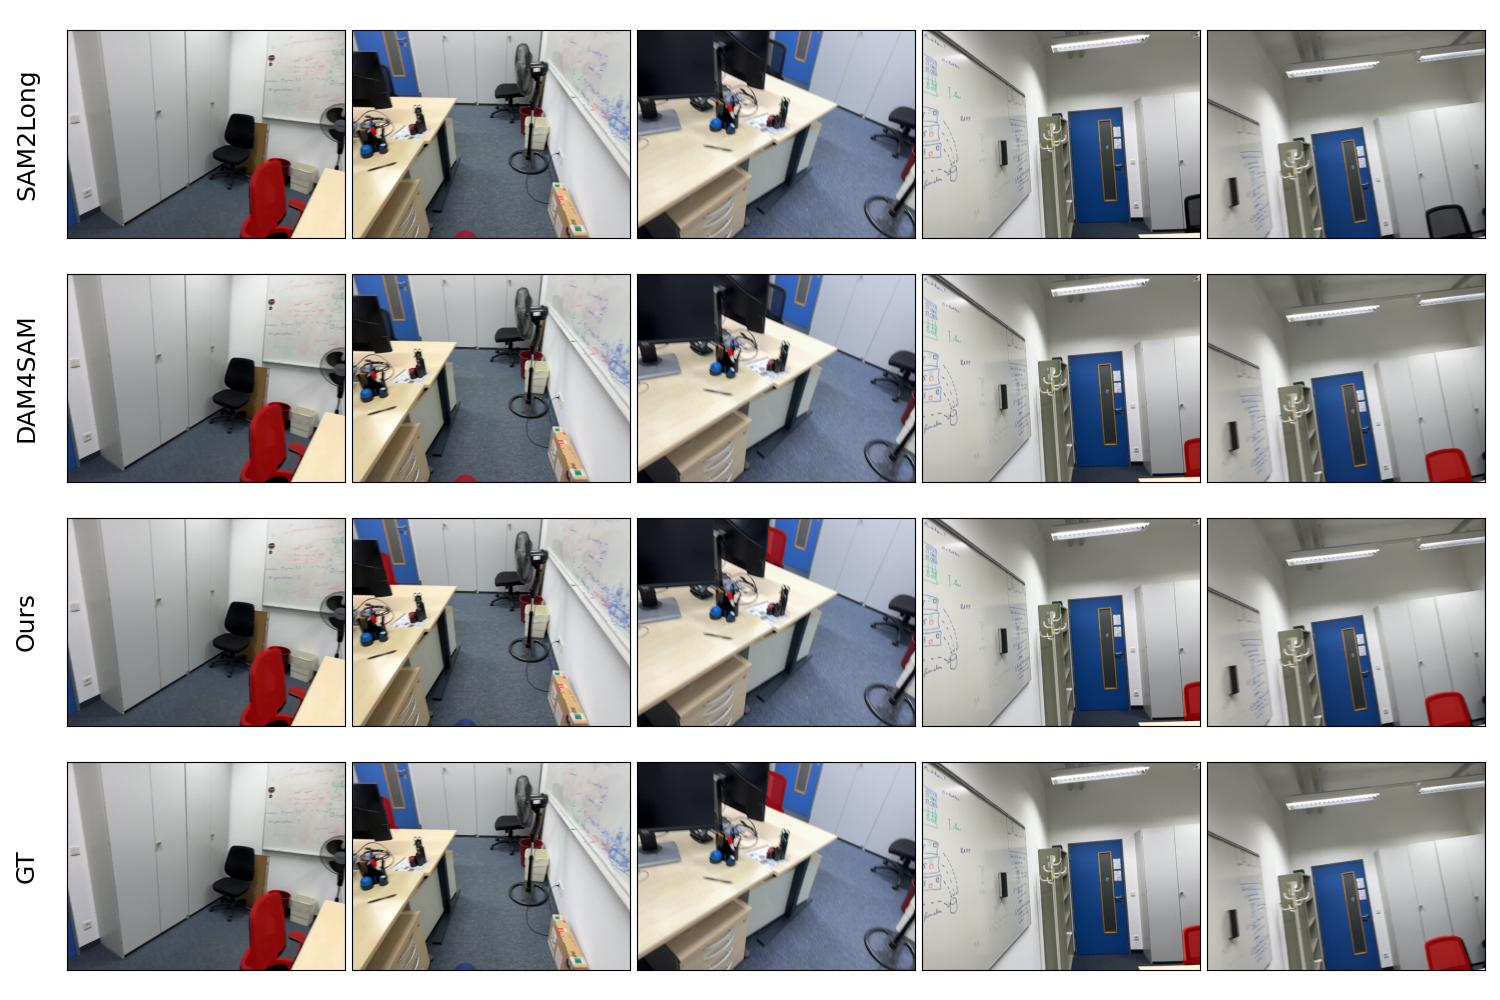
\includegraphics[width=1.0\textwidth]{figs/fig-vis/7b6477cb95/pred_masks_instance_512_53.jpg}
    \caption{
    \textbf{不同 VOS 方法的视觉比较}
    }
    \label{fig:vis_comp4}
\end{figure*}

\begin{figure*}[t]
    \centering
    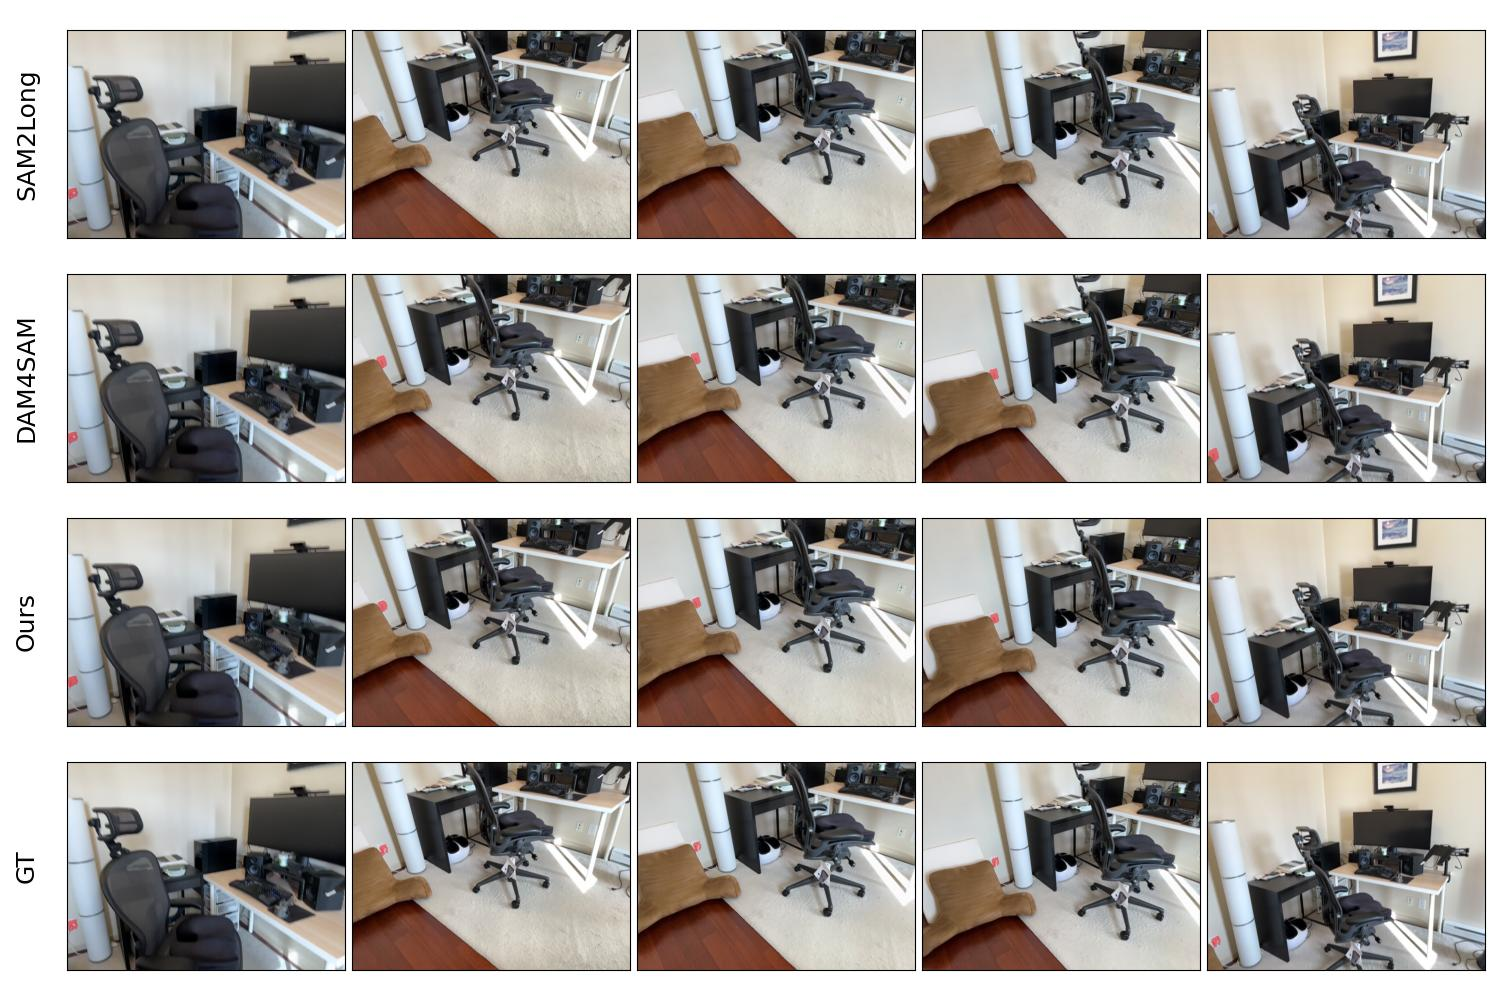
\includegraphics[width=1.0\textwidth]{figs/fig-vis/a24f64f7fb/pred_masks_instance_512_22.jpg}
    
\includegraphics[width=1.0\textwidth]{figs/fig-vis/acd95847c5/pred_masks_instance_512_10.jpg}
    \caption{
    \textbf{不同 VOS 方法的视觉比较}
    }
    \label{fig:vis_comp5}
\end{figure*}

\begin{figure*}[t]
    \centering
    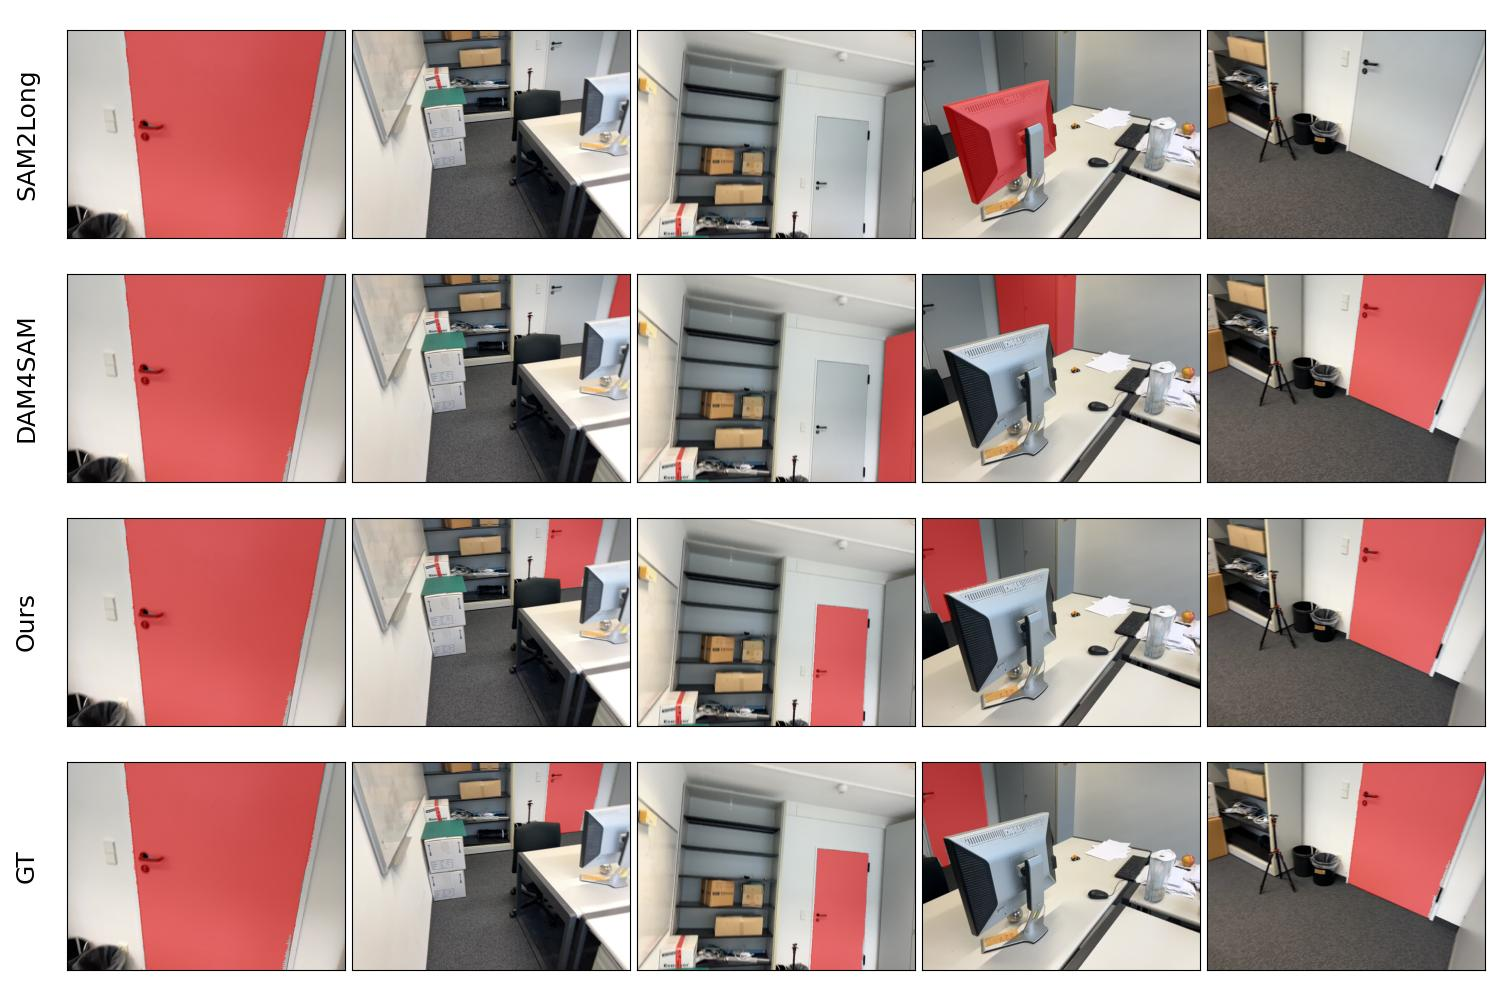
\includegraphics[width=1.0\textwidth]{figs/fig-vis/acd95847c5/pred_masks_instance_512_14.jpg}
    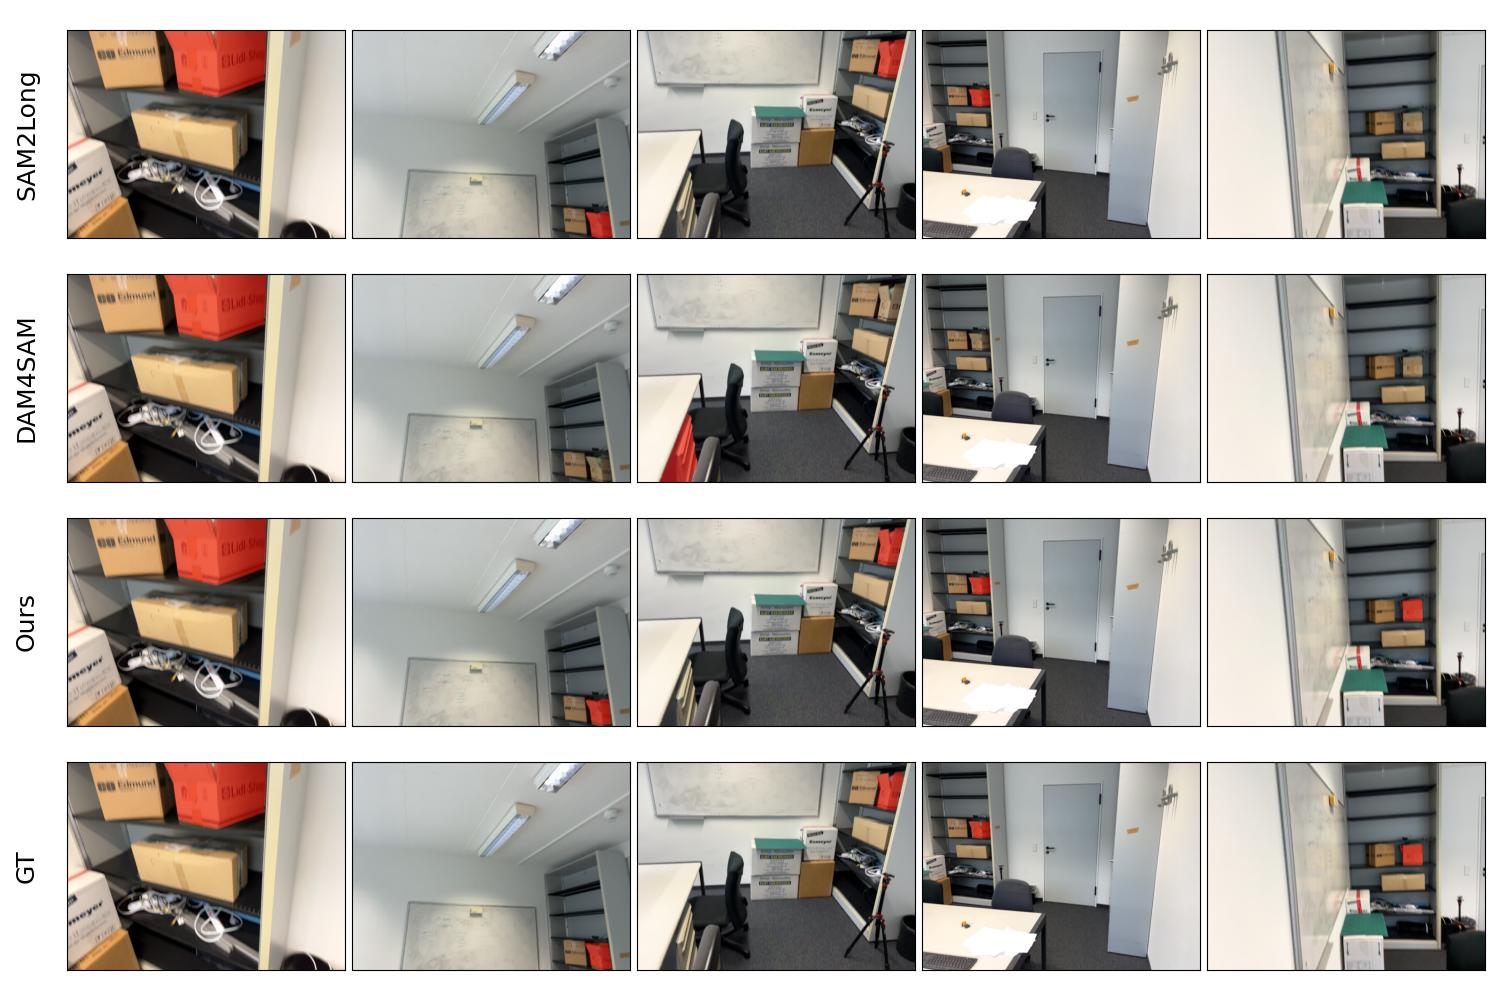
\includegraphics[width=1.0\textwidth]{figs/fig-vis/acd95847c5/pred_masks_instance_512_33.jpg}
    \caption{
    \textbf{不同 VOS 方法的视觉比较}
    }
    \label{fig:vis_comp6}
\end{figure*}

\begin{figure*}[t]
    \centering
    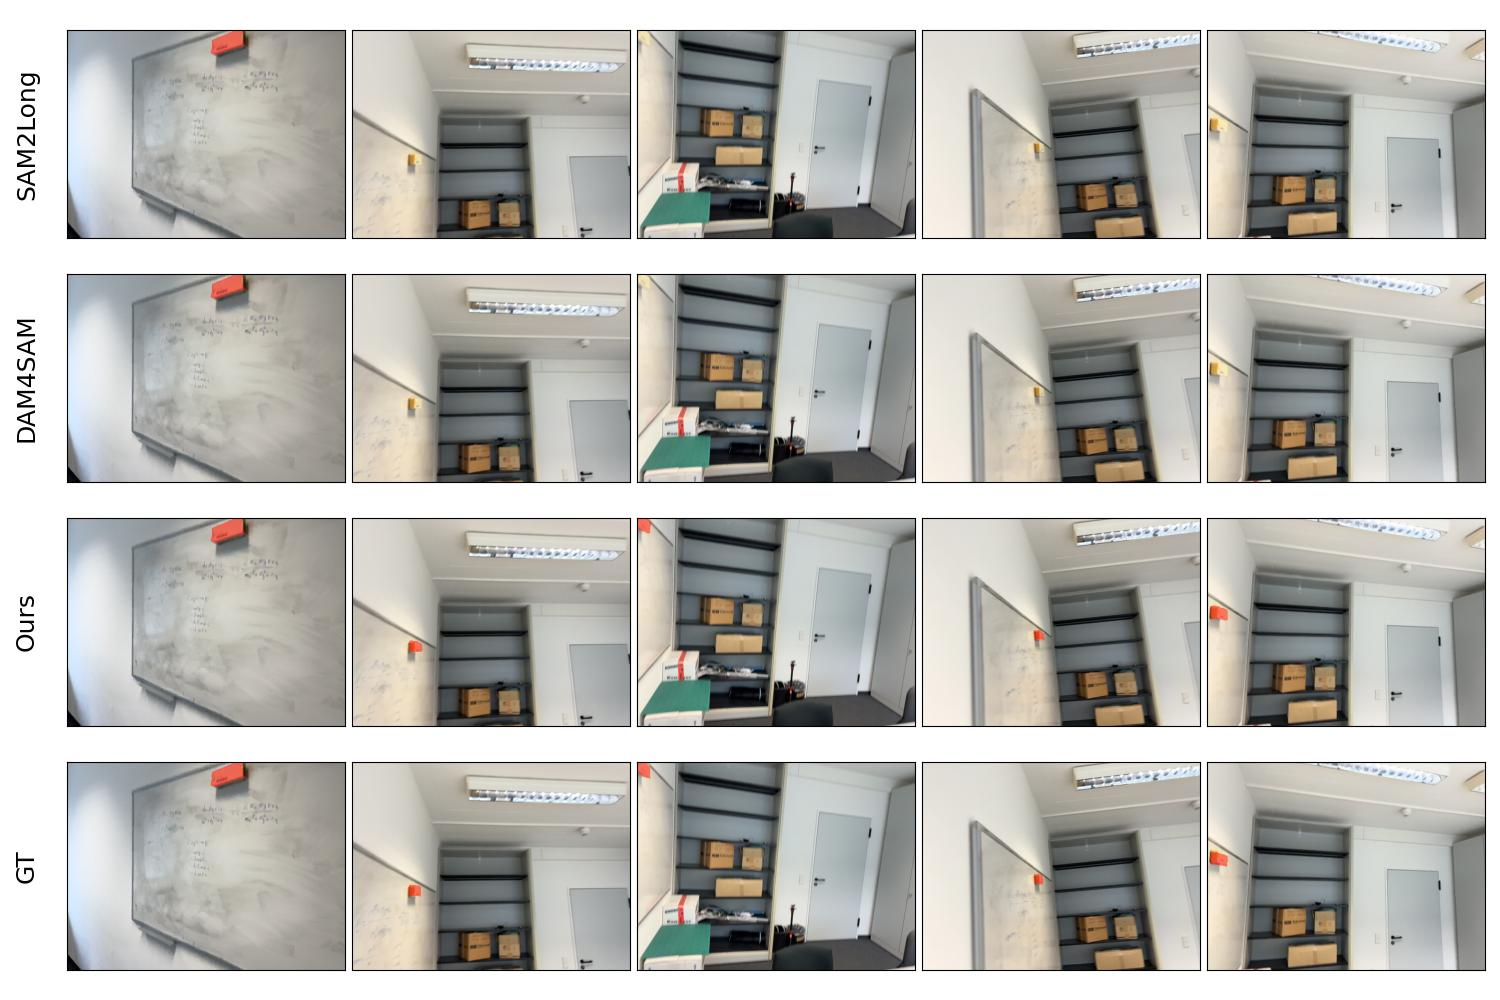
\includegraphics[width=1.0\textwidth]{figs/fig-vis/acd95847c5/pred_masks_instance_512_43.jpg}
    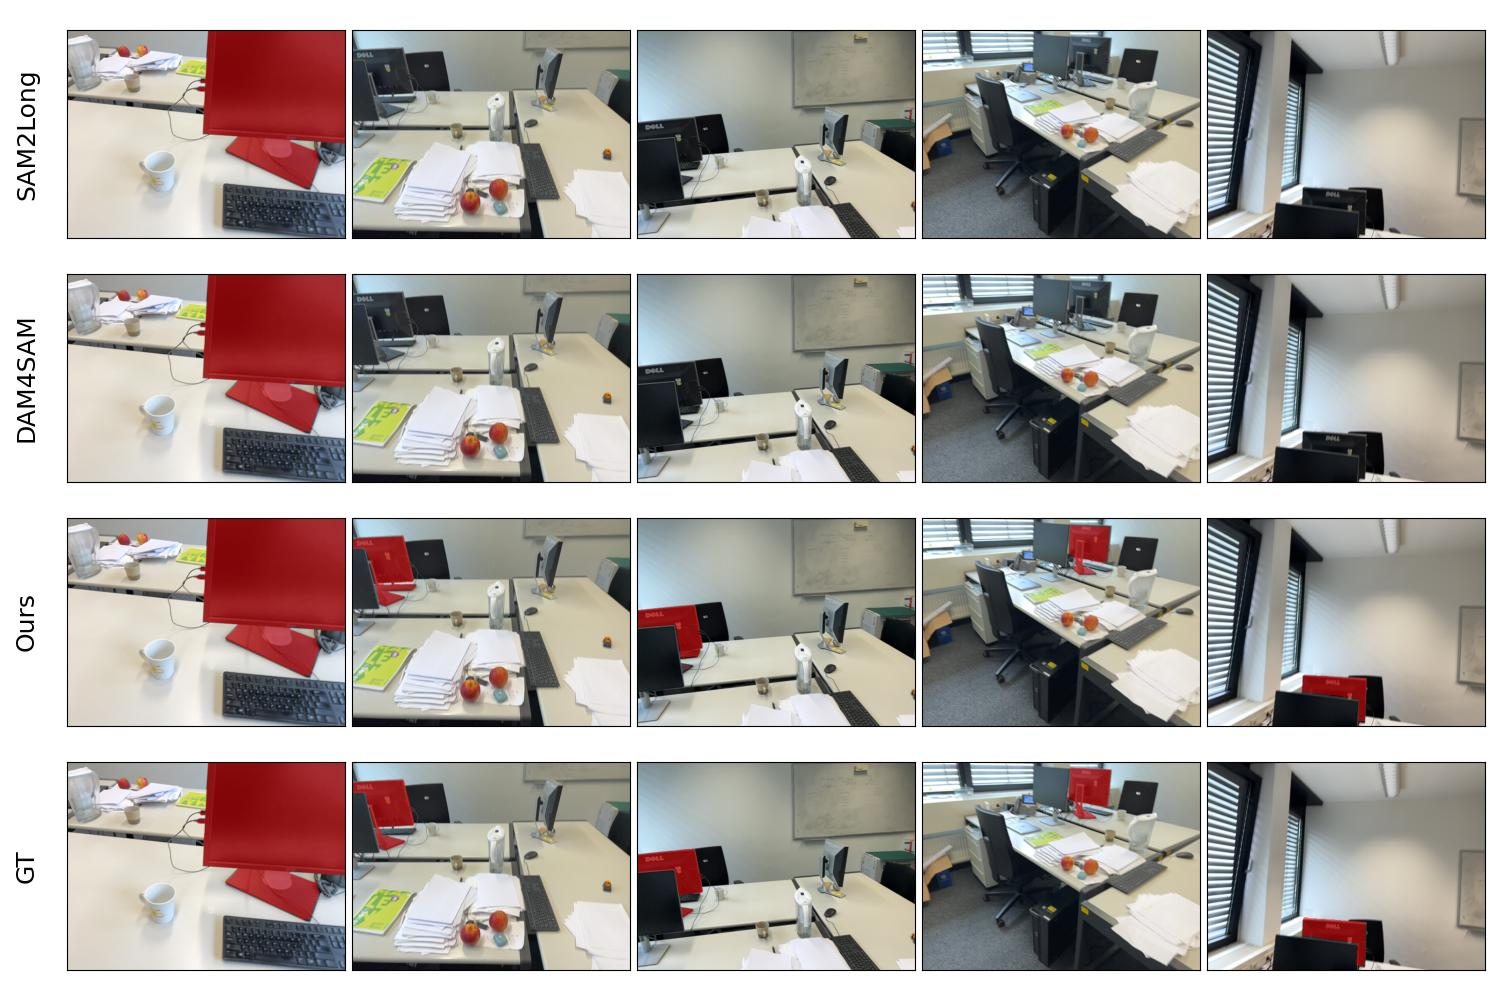
\includegraphics[width=1.0\textwidth]{figs/fig-vis/acd95847c5/pred_masks_instance_512_59.jpg}
    \caption{
    \textbf{不同 VOS 方法的视觉比较}
    }
    \label{fig:vis_comp7}
\end{figure*}

\section{定性比较} \label{sec:more_qualitative}
\paragraph{视频比较}
我们在 \cref{fig:vis_comp,fig:vis_comp2,fig:vis_comp3,fig:vis_comp4,fig:vis_comp5,fig:vis_comp6,fig:vis_comp7} 中提供视频对象跟踪可视化。
\paragraph{类别无关实例分割。}
我们在~\cref{fig:visual_class} 中提供类别无关实例分割的额外视觉结果。




\begin{figure*}[ht]
\centering
\small
\setlength{\tabcolsep}{2pt}
\resizebox{\textwidth}{!}{
\begin{tabular}{ccc}
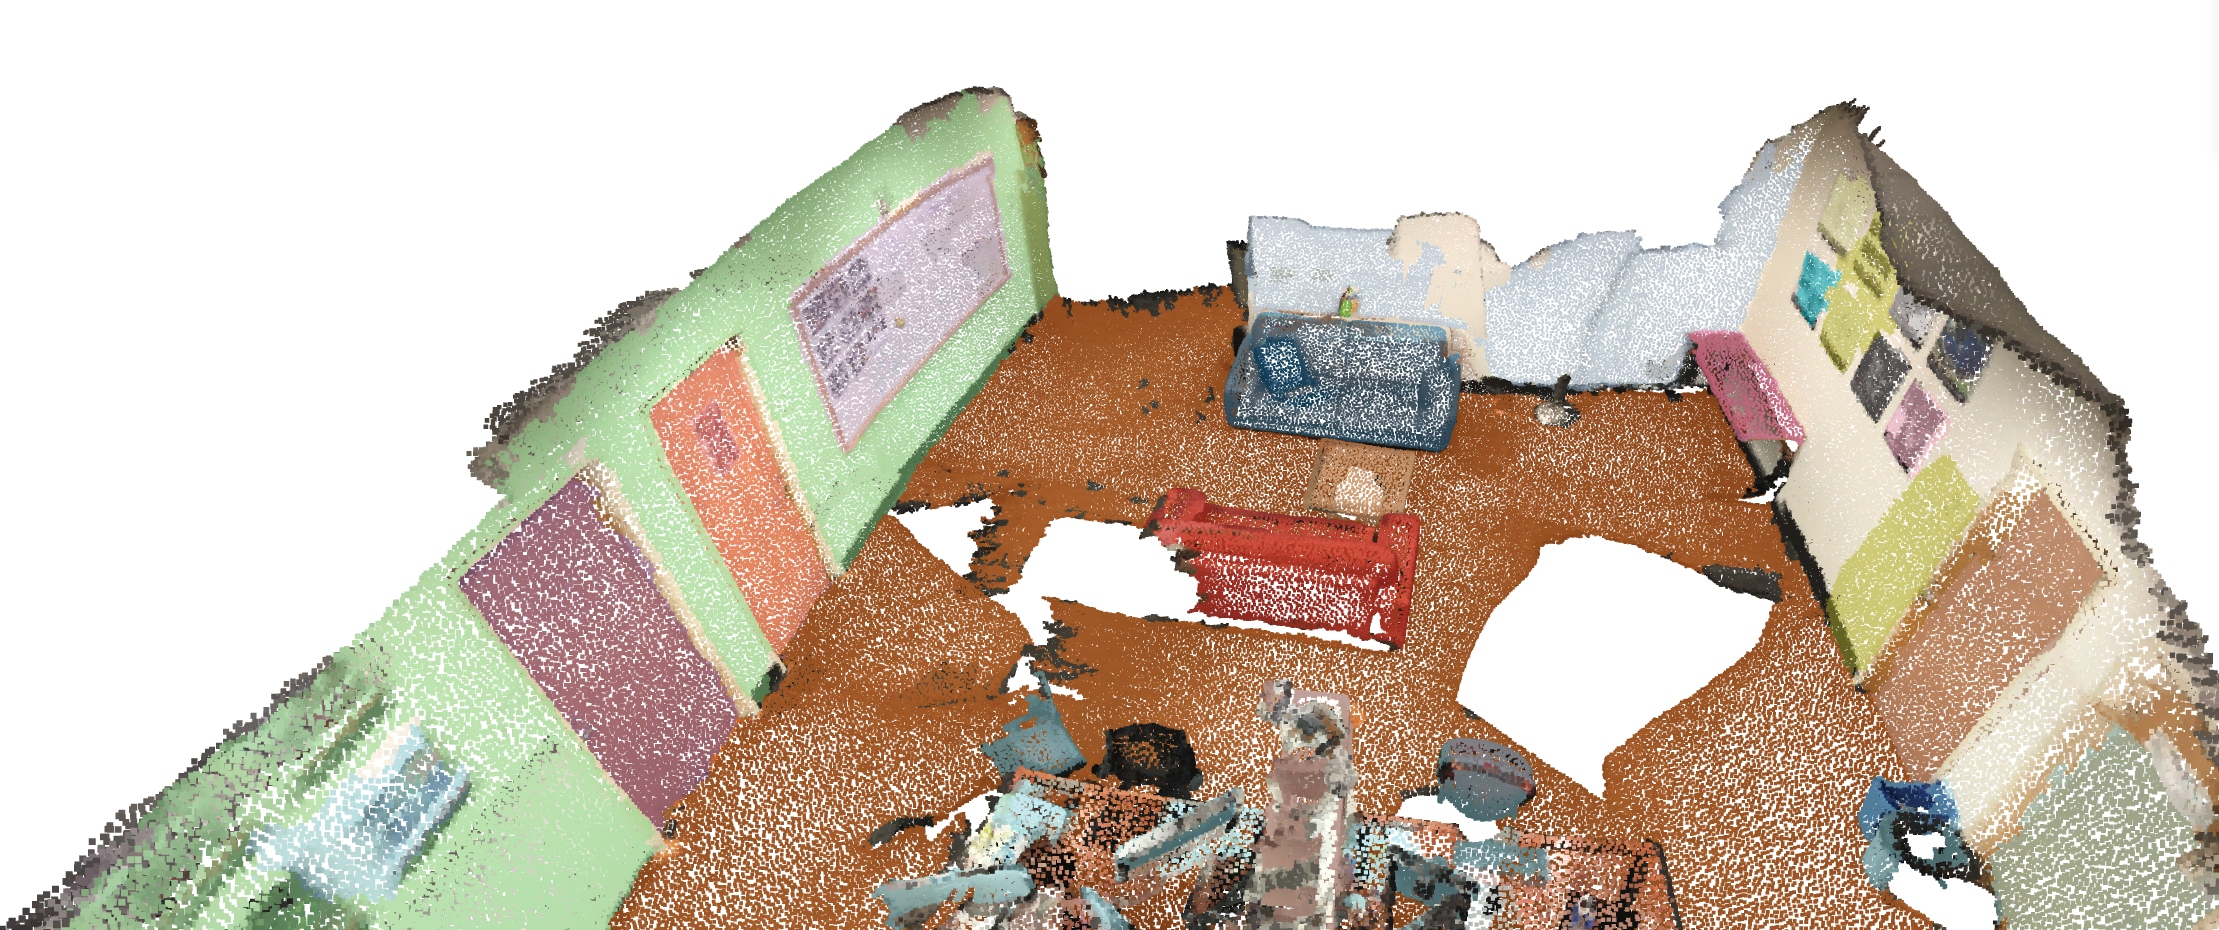
\includegraphics[width=0.33\textwidth]{figs/3D-Visual/1_1.png} & 
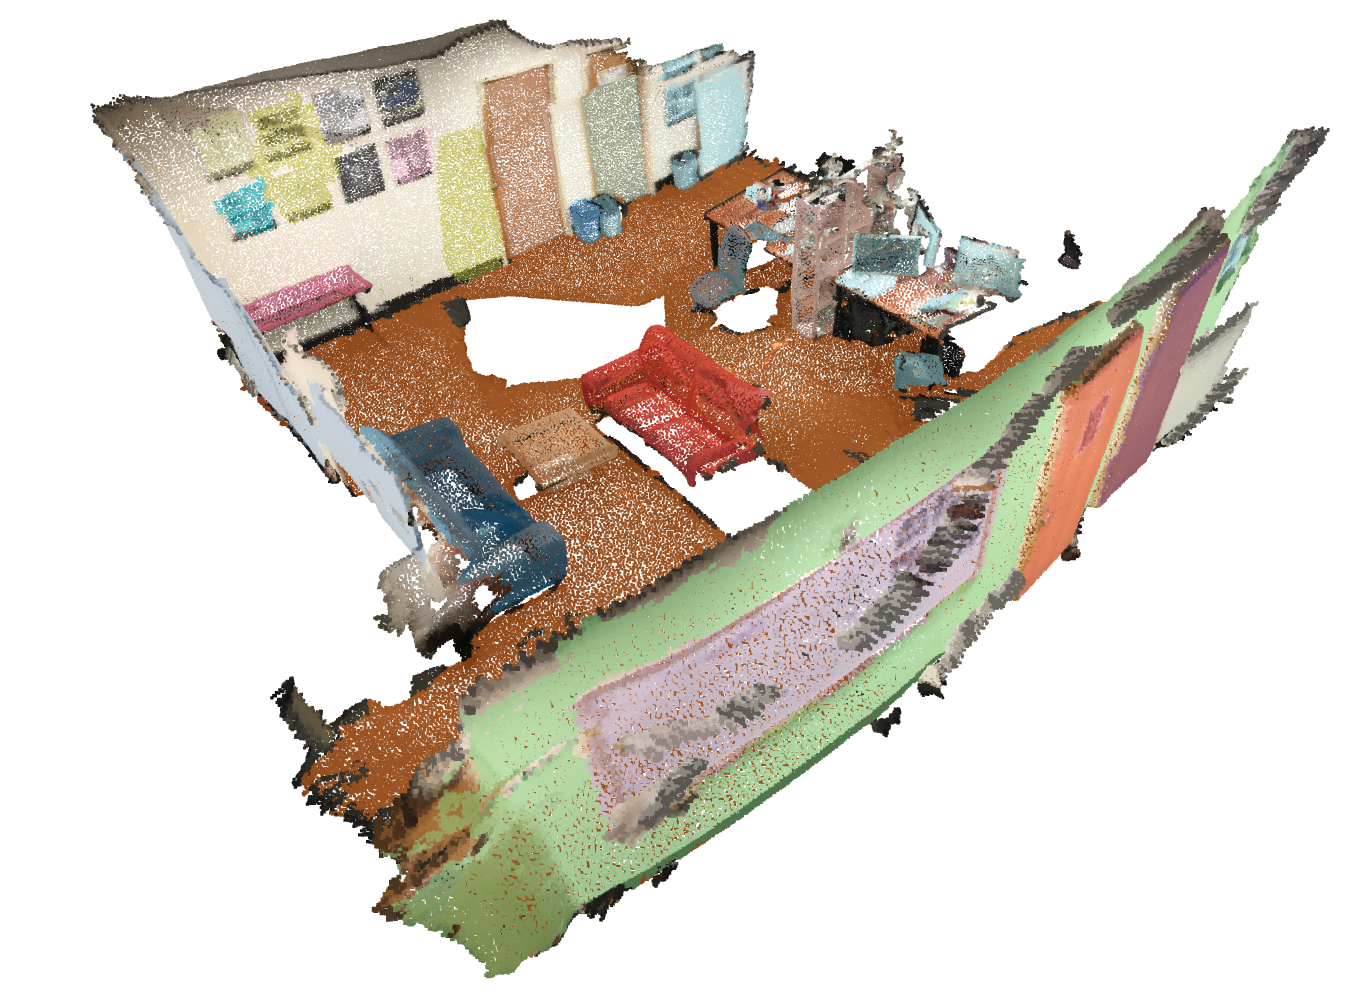
\includegraphics[width=0.33\textwidth]{figs/3D-Visual/1_2.png} & 
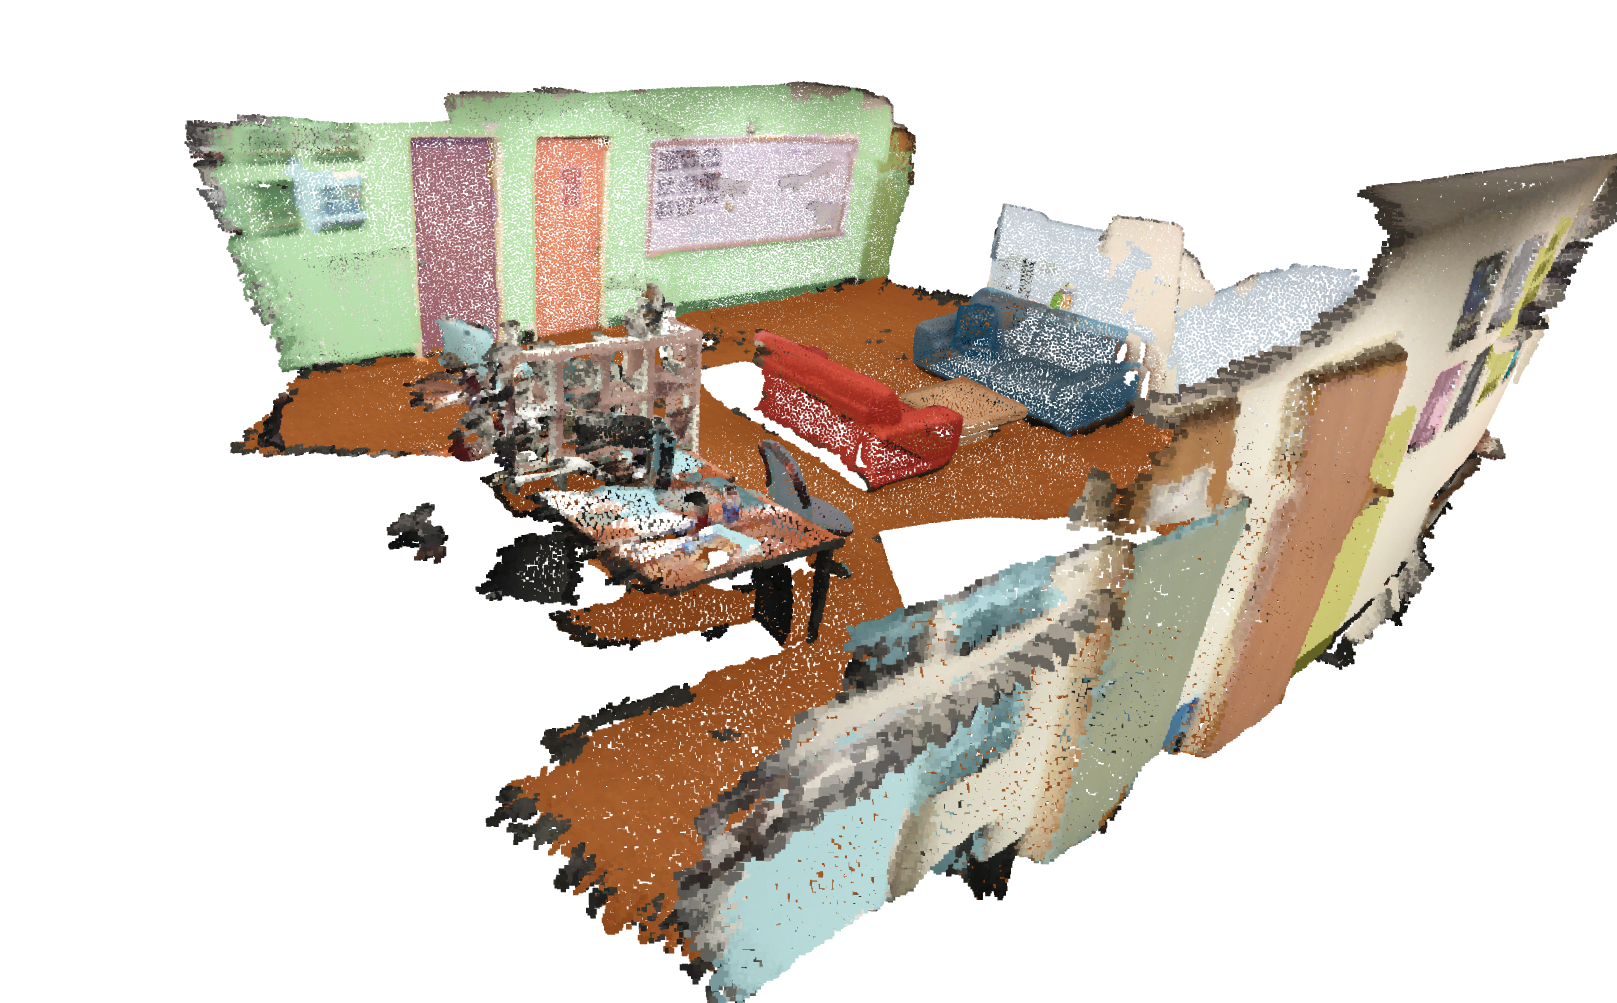
\includegraphics[width=0.33\textwidth]{figs/3D-Visual/1_3.png} \\
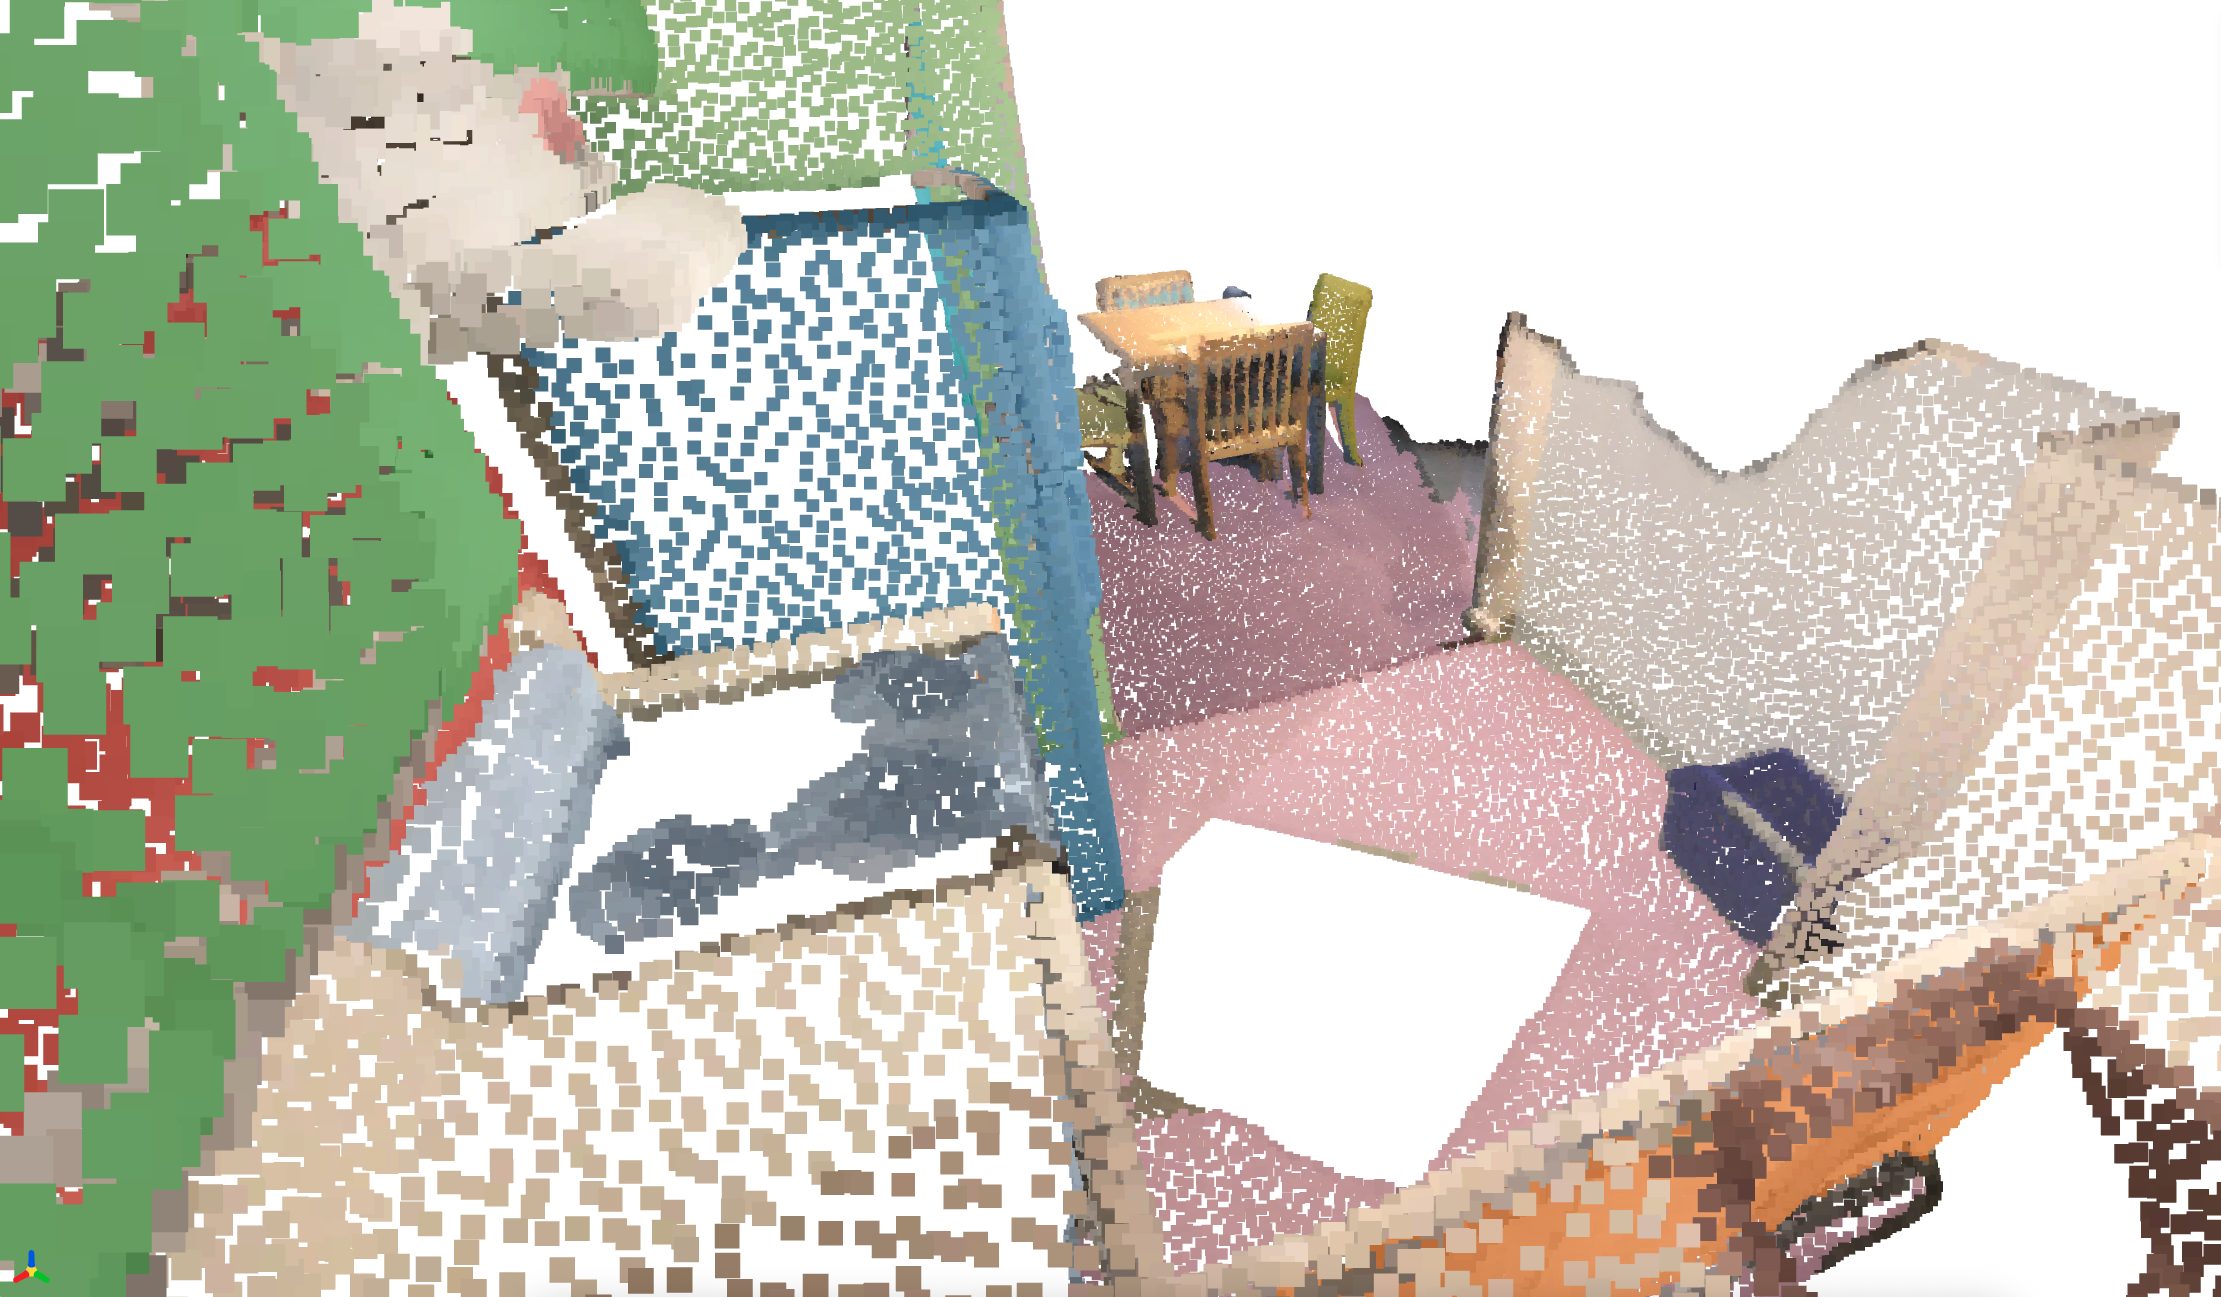
\includegraphics[width=0.33\textwidth]{figs/3D-Visual/2_1.png} & 
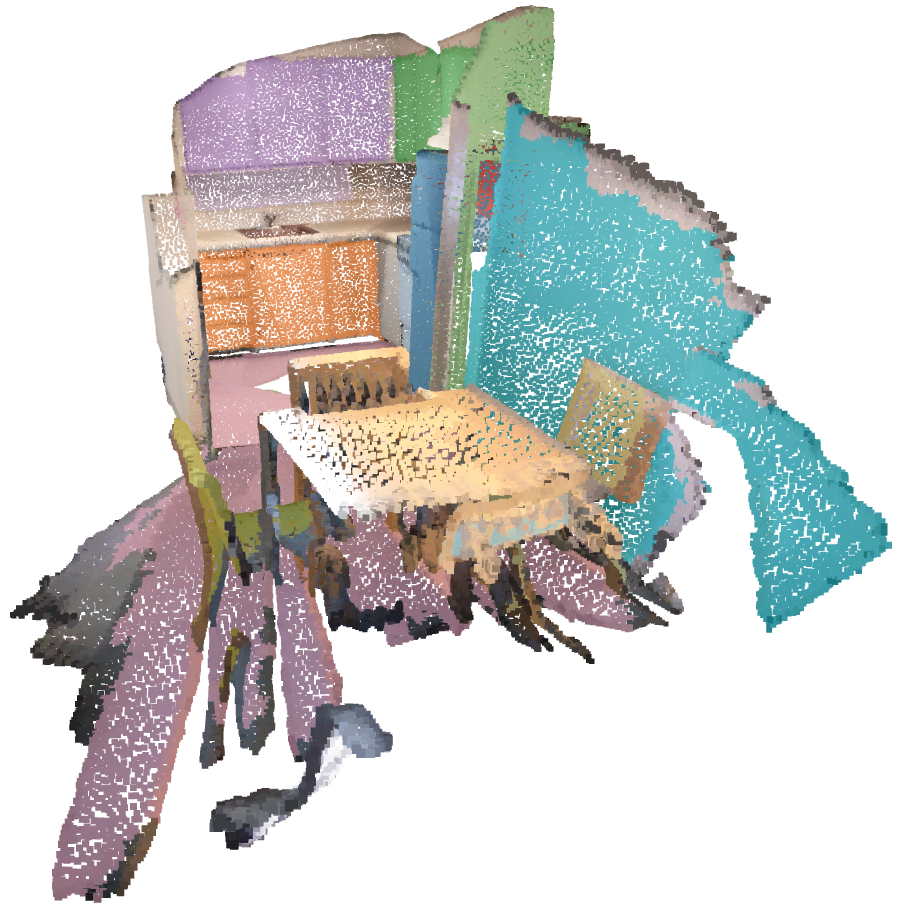
\includegraphics[width=0.33\textwidth]{figs/3D-Visual/2_2.png} & 
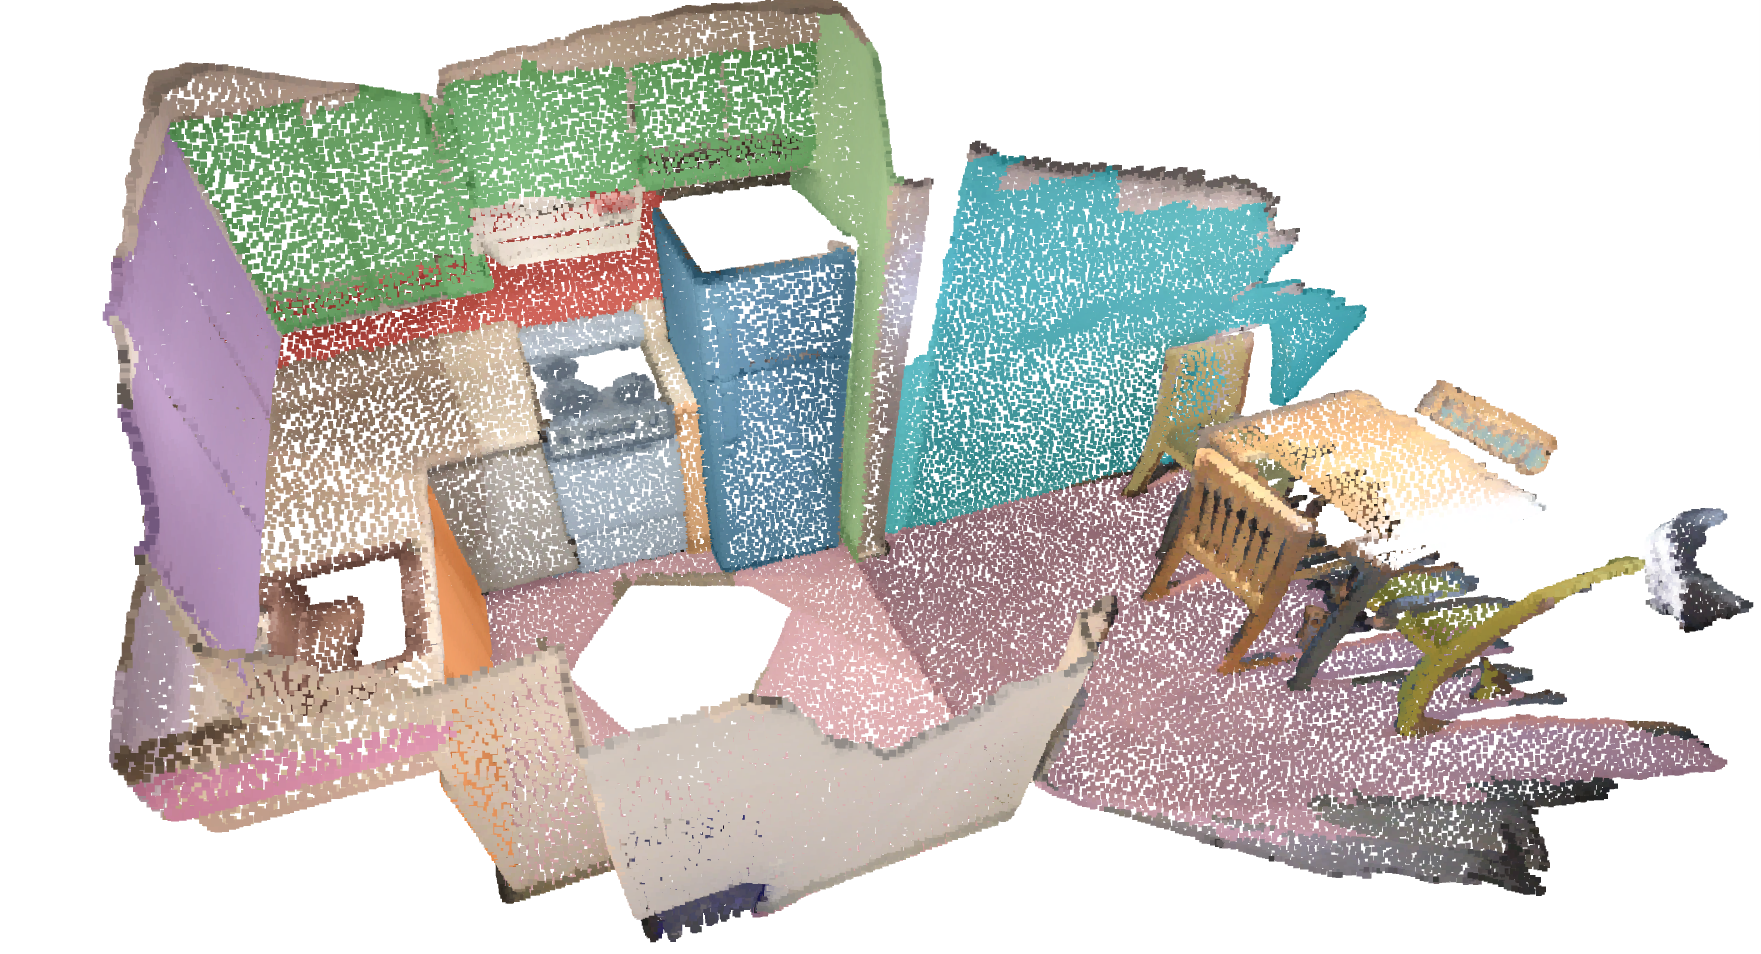
\includegraphics[width=0.33\textwidth]{figs/3D-Visual/2_3.png} \\
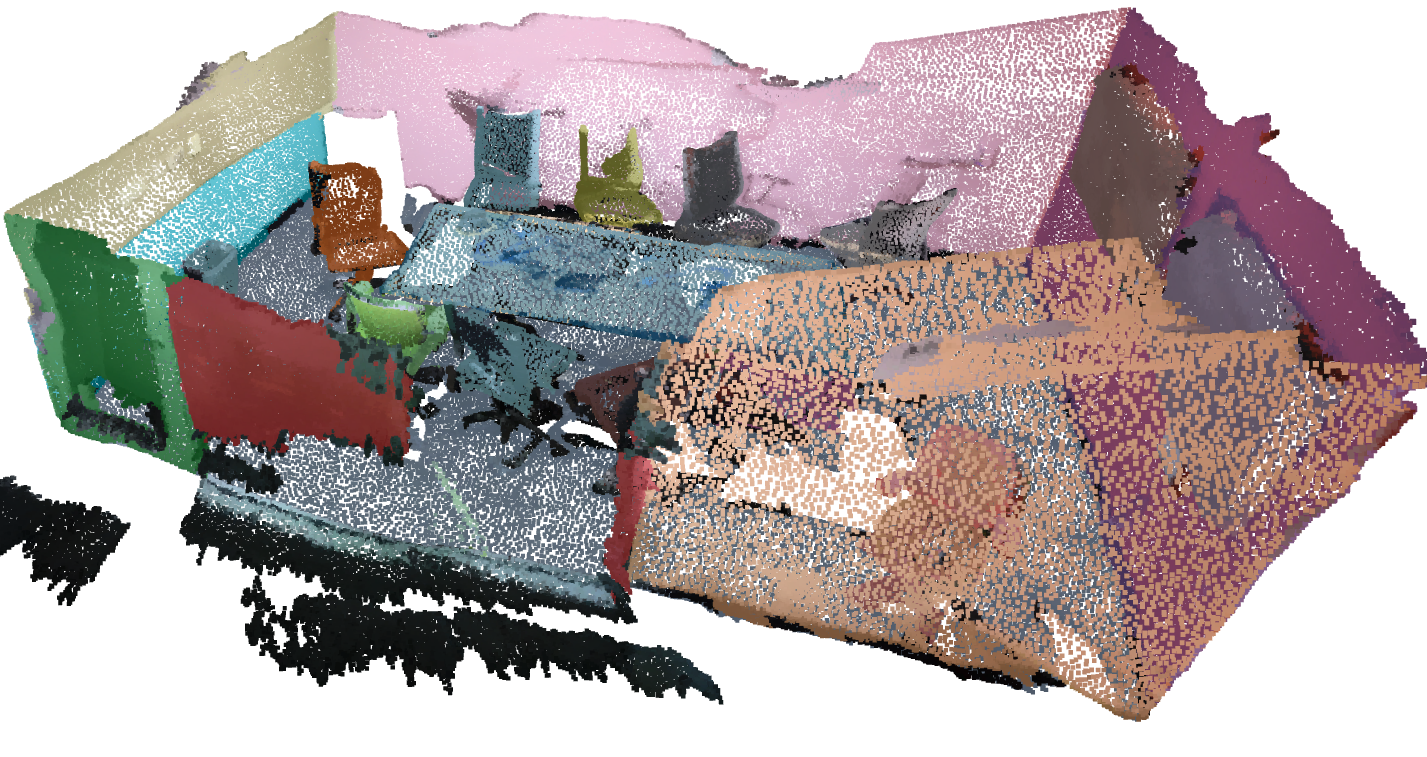
\includegraphics[width=0.33\textwidth]{figs/3D-Visual/3_1.png} & 
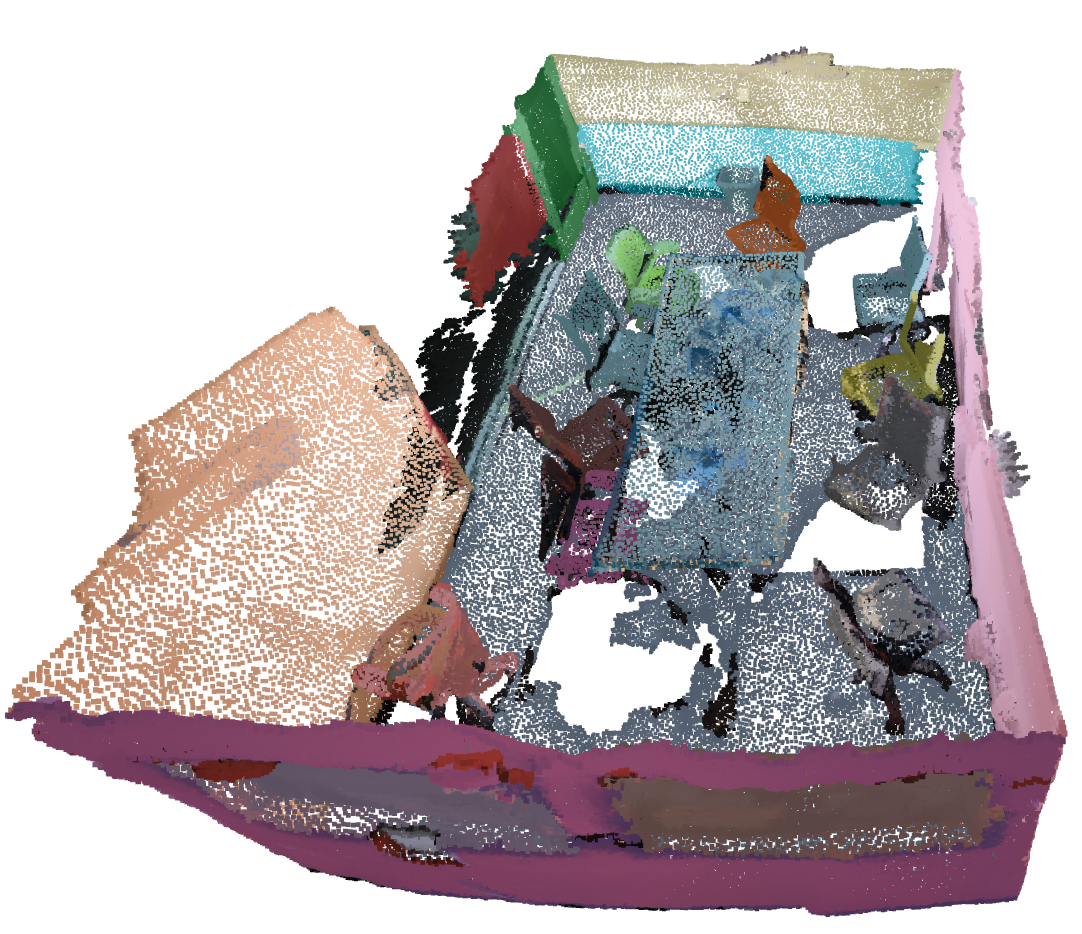
\includegraphics[width=0.33\textwidth]{figs/3D-Visual/3_2.png} & 
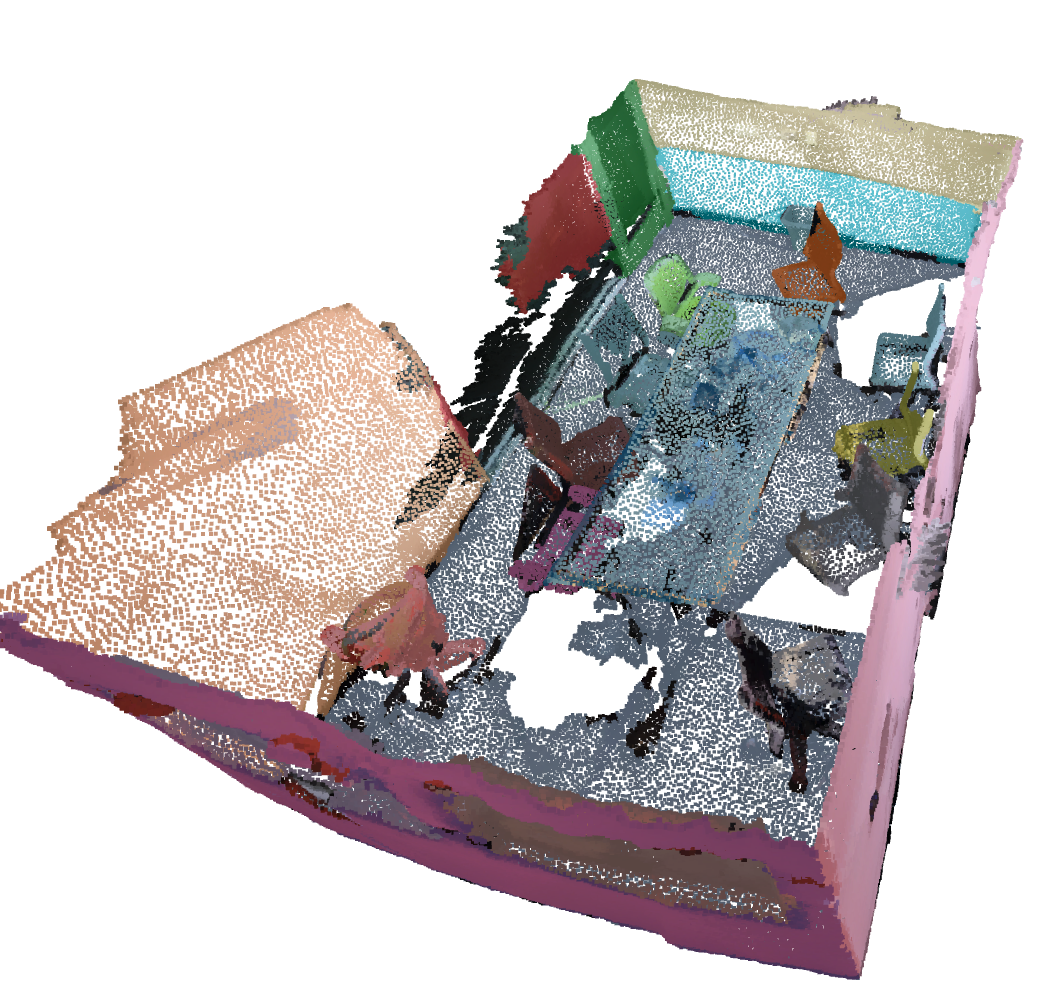
\includegraphics[width=0.33\textwidth]{figs/3D-Visual/3_3.png} \\
\end{tabular}
}
\caption{
\textbf{类别无关实例分割的视觉结果。}
}
\label{fig:visual_class}
\end{figure*}
